\beginsupplement

\section[Supplementary figures]{Supplementary figures}
\label{sec:supp_fig}

\subsection{XGBoost classifier to uncover the function of lncRNAs in cell-growth}
\label{sec:sup_fig_part_2}

\begin{figure}[!htb]
  \centering
  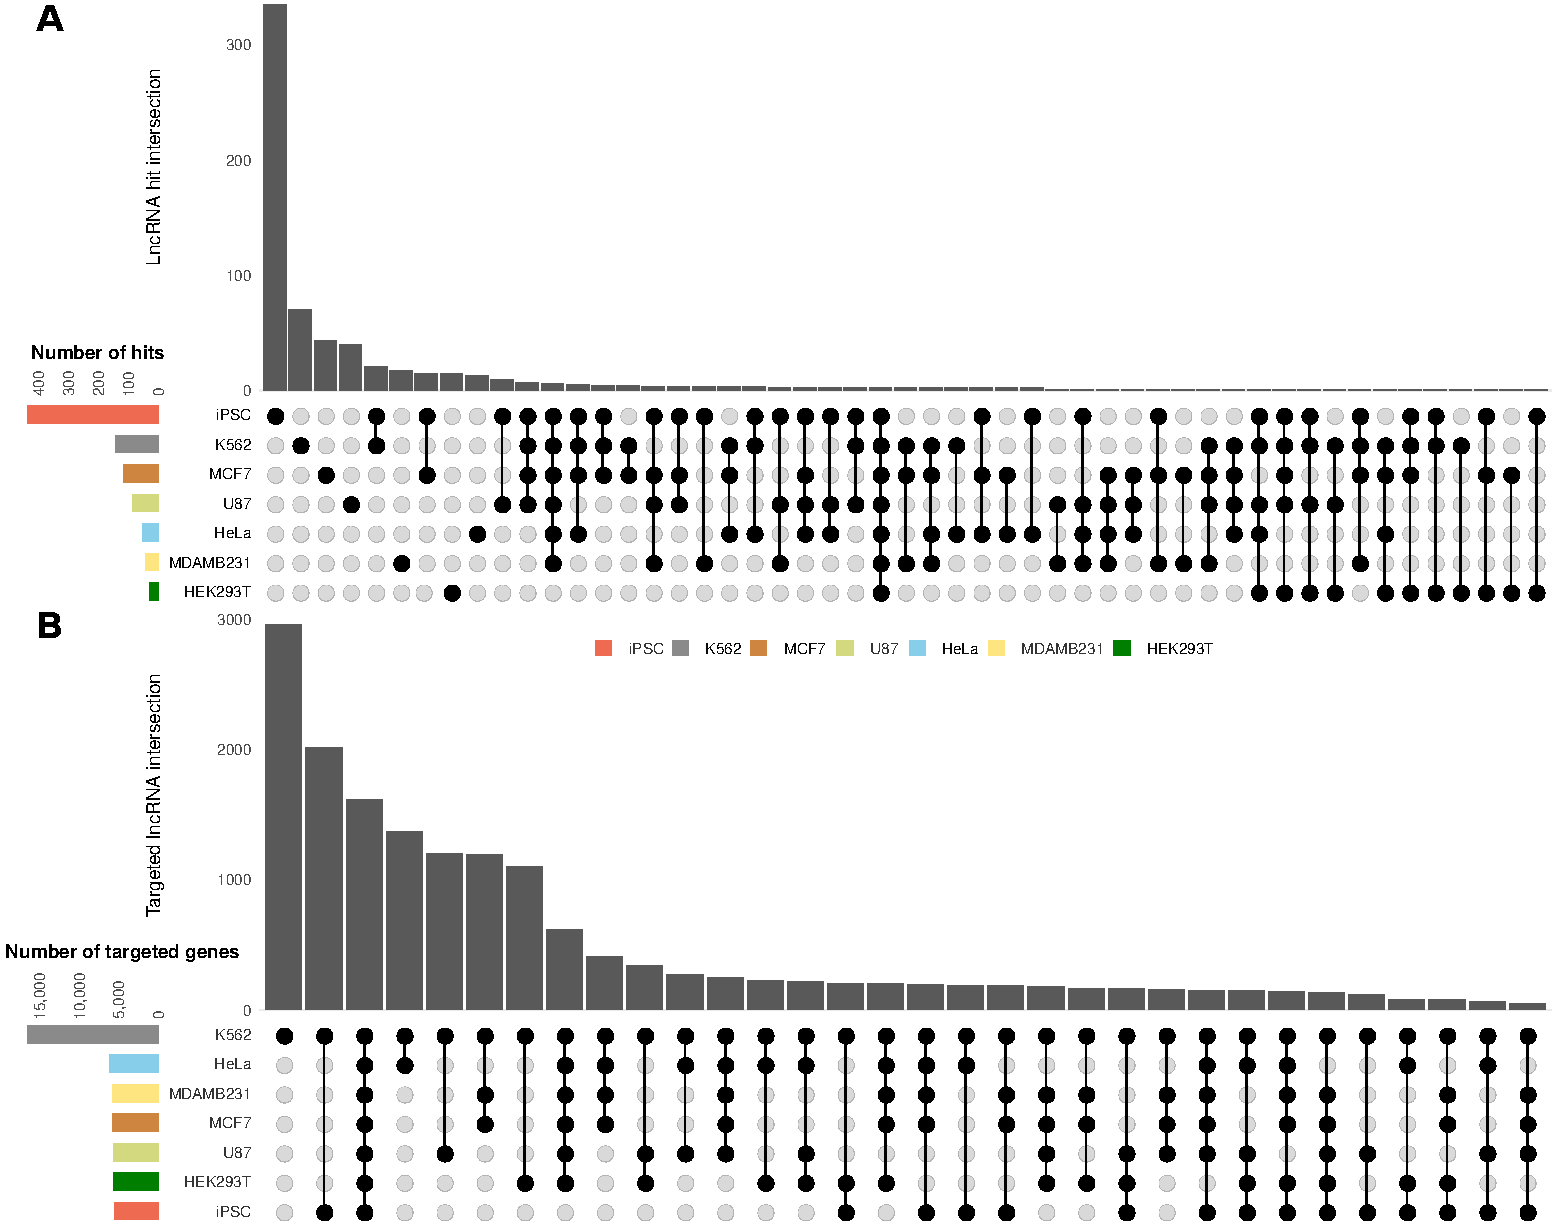
\includegraphics[scale=0.44]{plots/appendix/ml/hits.lncRNAs.intersections.pdf}
  \caption[Intersections of hits and targeted genes]{\textbf{Intersections of hits and targeted genes}. \textbf{(A)} LncRNA hits intersections. \textbf{(B)} Intersection of targeted lncRNAs from CRISPRi dataset.  Vertical bars represent the number of hits and targeted lncRNAs, respectively. Number of hits and lncRNAs are indicated in the horizontal bars.}
  \label{supp-fig:hit-lncRNA-intersection}
\end{figure}

The following figure represents  \textit{UCSC} genome browser plots of two transcript hit examples in hg19 assembly version. Exons are represented as solid red boxes, introns are depicted as thin arrowed lines and black boxes represent the selected promoters.

\begin{figure}[!htb]
    \centering
    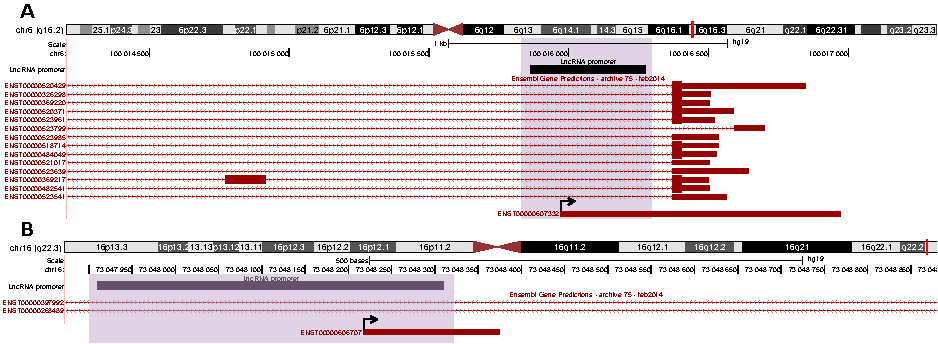
\includegraphics[width=0.98\textwidth]{img/appendix/appendix_fig/ml/ucsc.lncRNA.promoters.v2.pdf}
    \caption[\textit{UCSC} promoter plots]{\textbf{\textit{UCSC} promoter plots}. \textbf{(A)} \textit{ENST00000607332} transcript on the positive strand. \textbf{(B)} \textit{ENST00000606707} on the negetive strand. Purple shaded regions denote promoter regions.}
    \label{supp-fig:ucsc_promoters_examples}
\end{figure}

\begin{figure}[!htb]
  \centering
  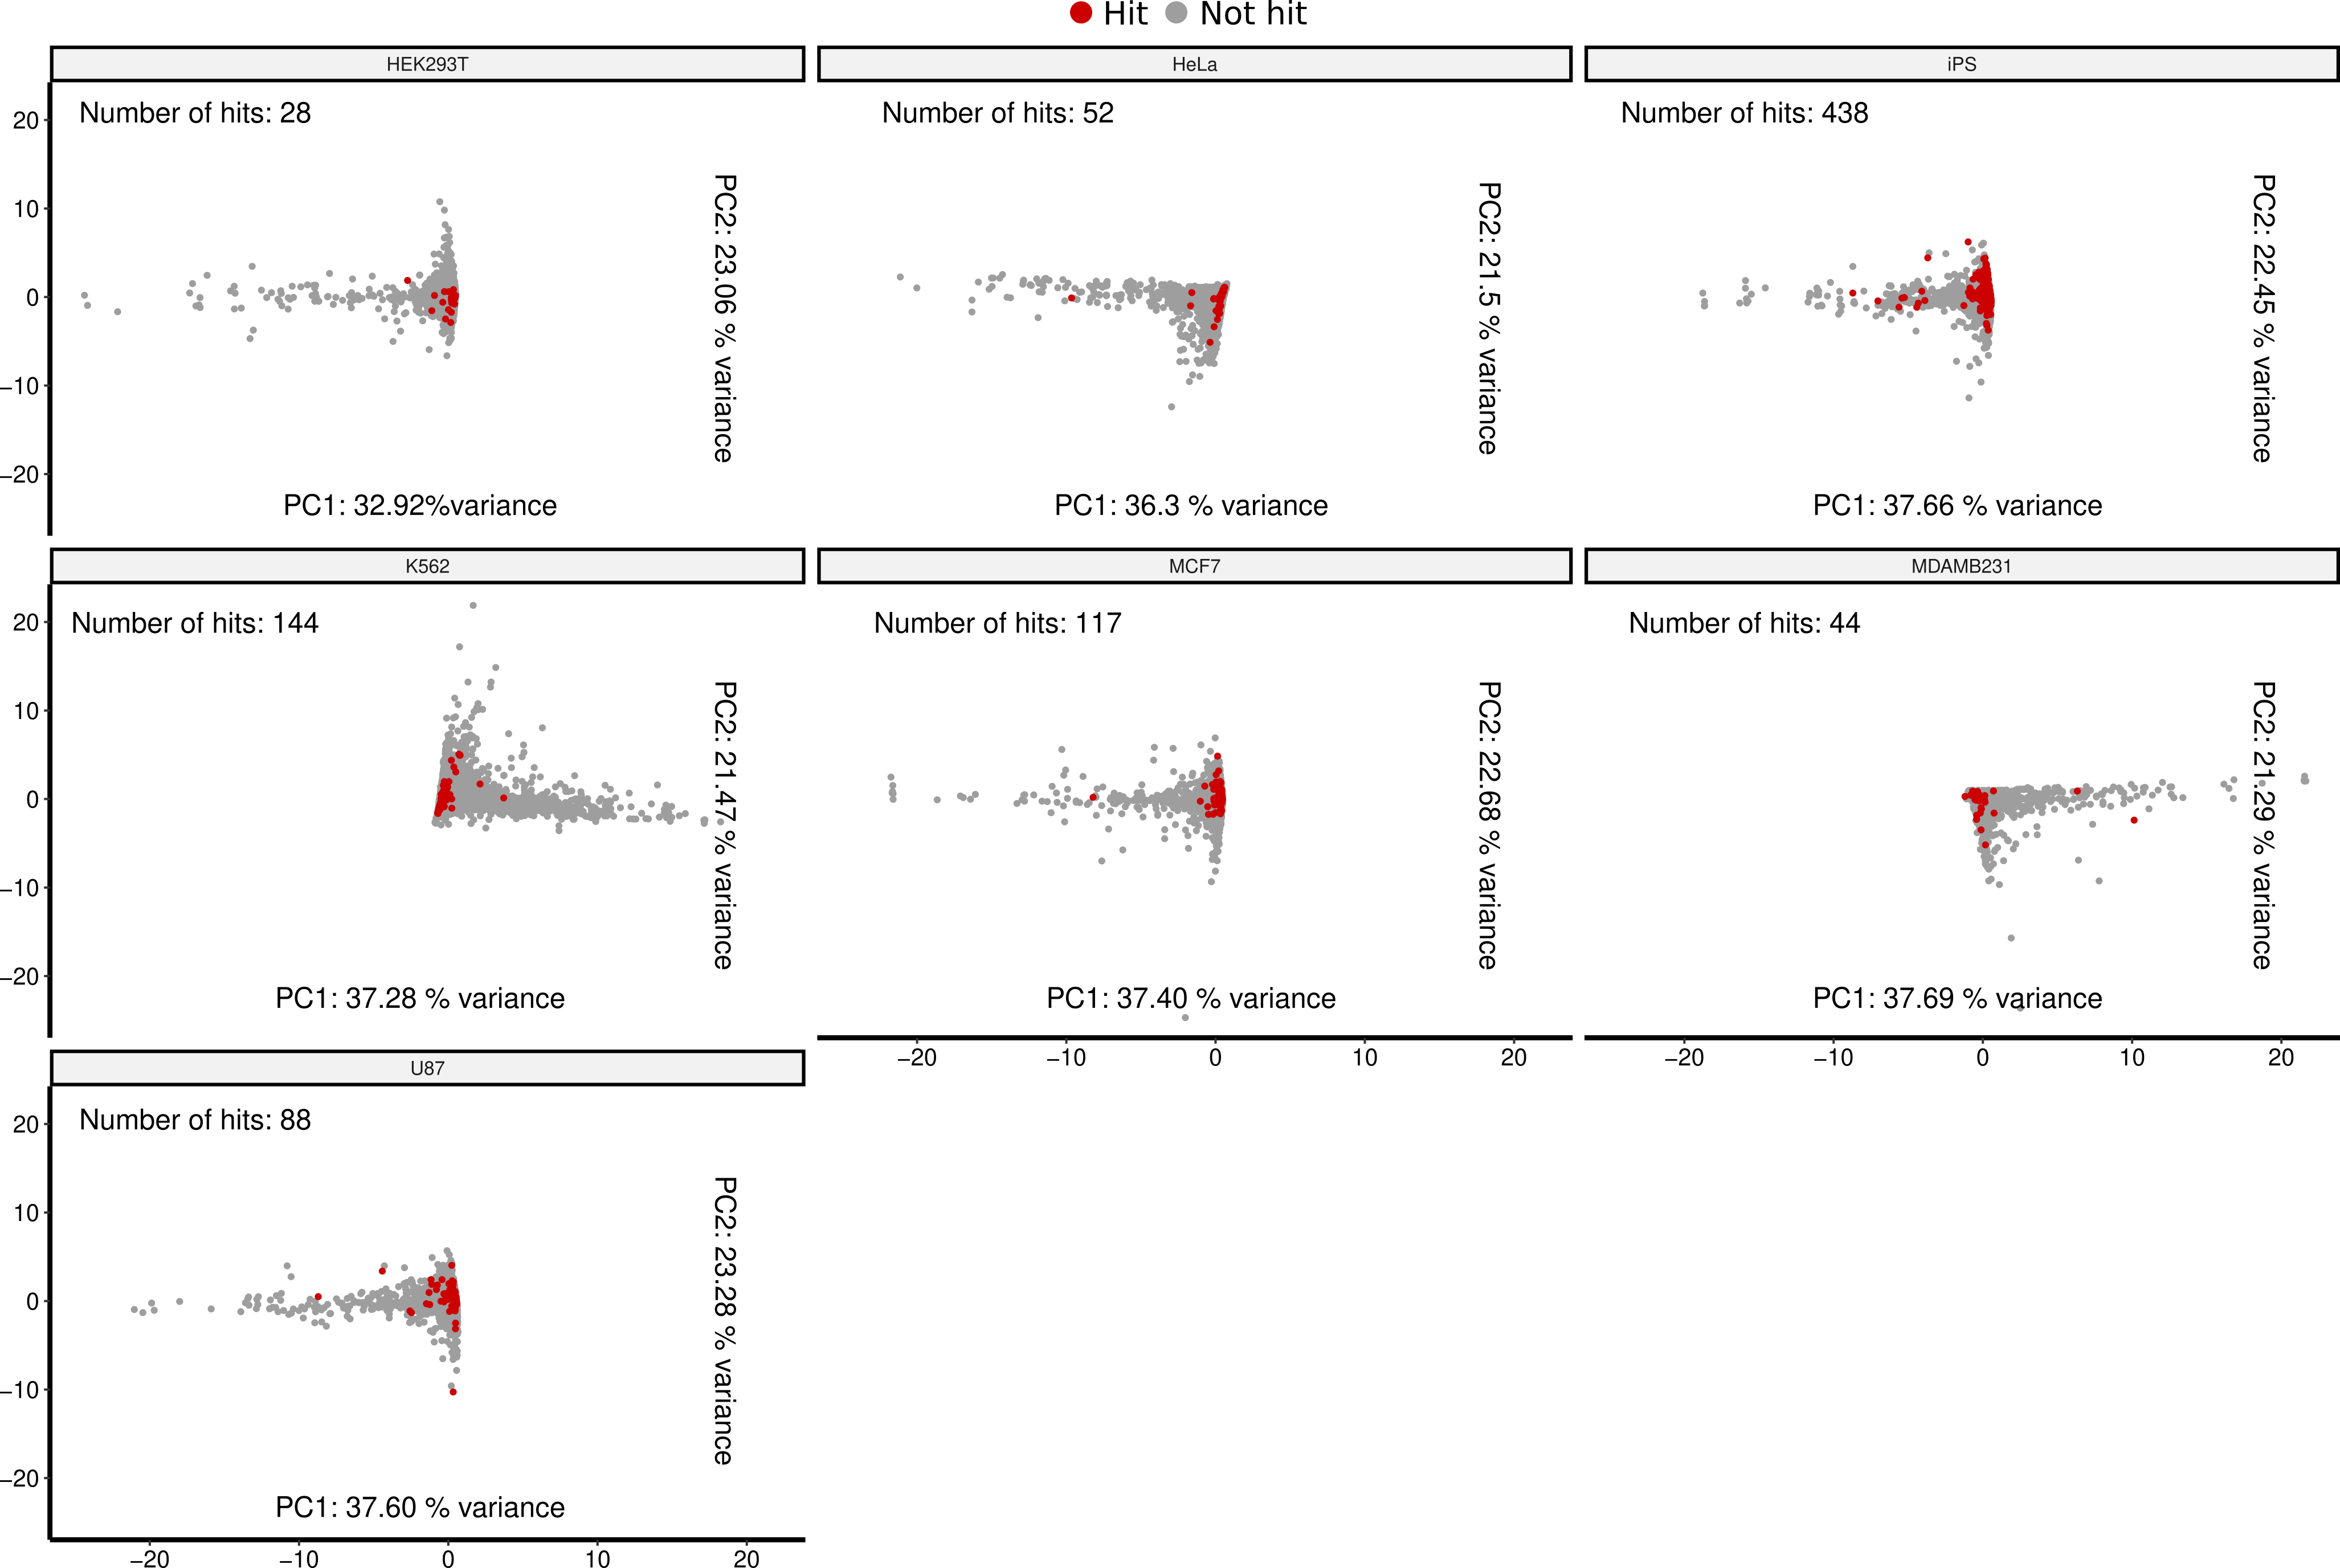
\includegraphics[width=0.9\textwidth]{plots/appendix/ml/pca.hit.percell.png}
  \caption[PCA of CRISPRi data]{\textbf{PCA of CRISPRi data}. PCA based on the 5 numeric variables from the 18 CRISPIRi features. (Expression level, number of exons, transcript length, locus locus distance, and TSS PC distance). Red dots= hit; grey dots= not hit.}
  \label{fig:pca-hits}
\end{figure}

\begin{figure}[ht!]
  \centering
  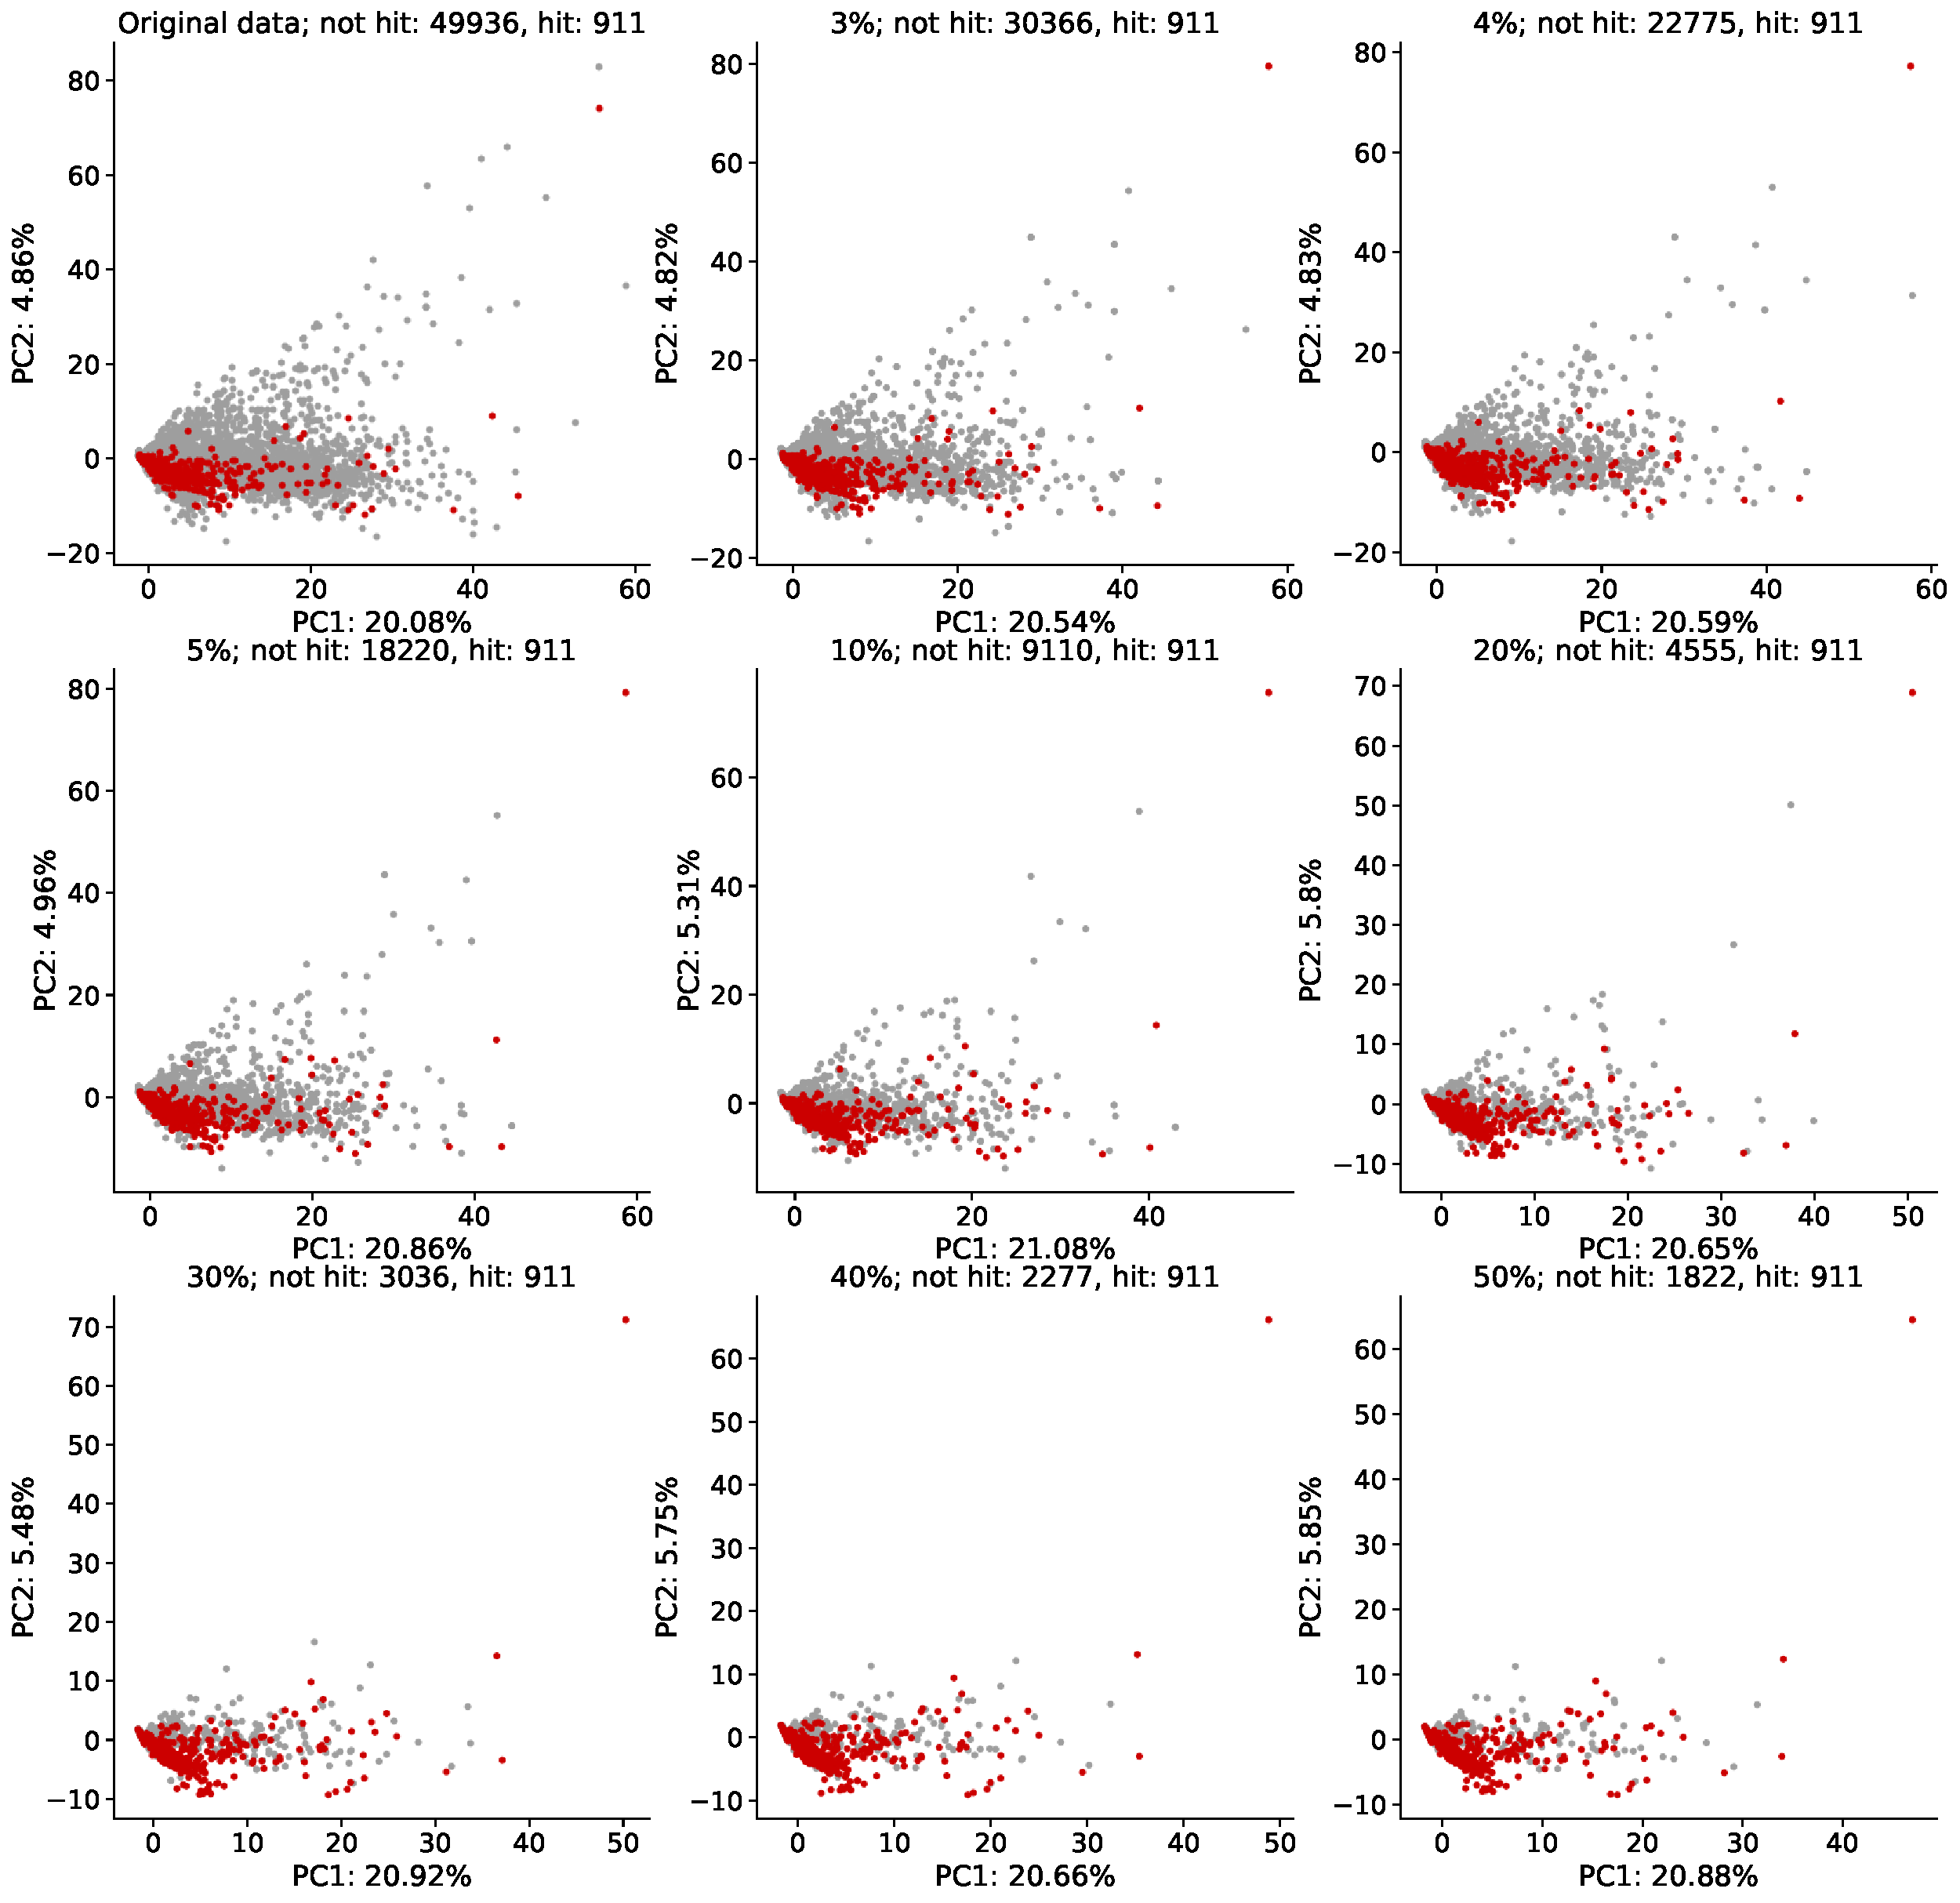
\includegraphics[scale=0.3]{plots/appendix/ml/pca.random.us.with.replacement.pdf}
  \caption[Under-sampling with replacement PCA]{\textbf{Under-sampling with replacement PCA}. PCA of random under-sampling of the majority class (\textit{i.e.} not hit) with replacement, plotting the complete dataset (upper-left plot) plus 8 sampling strategies. PCA values based on 130 numeric features showing the removed not hit transcripts. Red dots= hit; grey dots= not hit.}
  \label{supp-fig:pca-under-sampling-with-r}
\end{figure}

\begin{figure}[!htb]
  \centering
  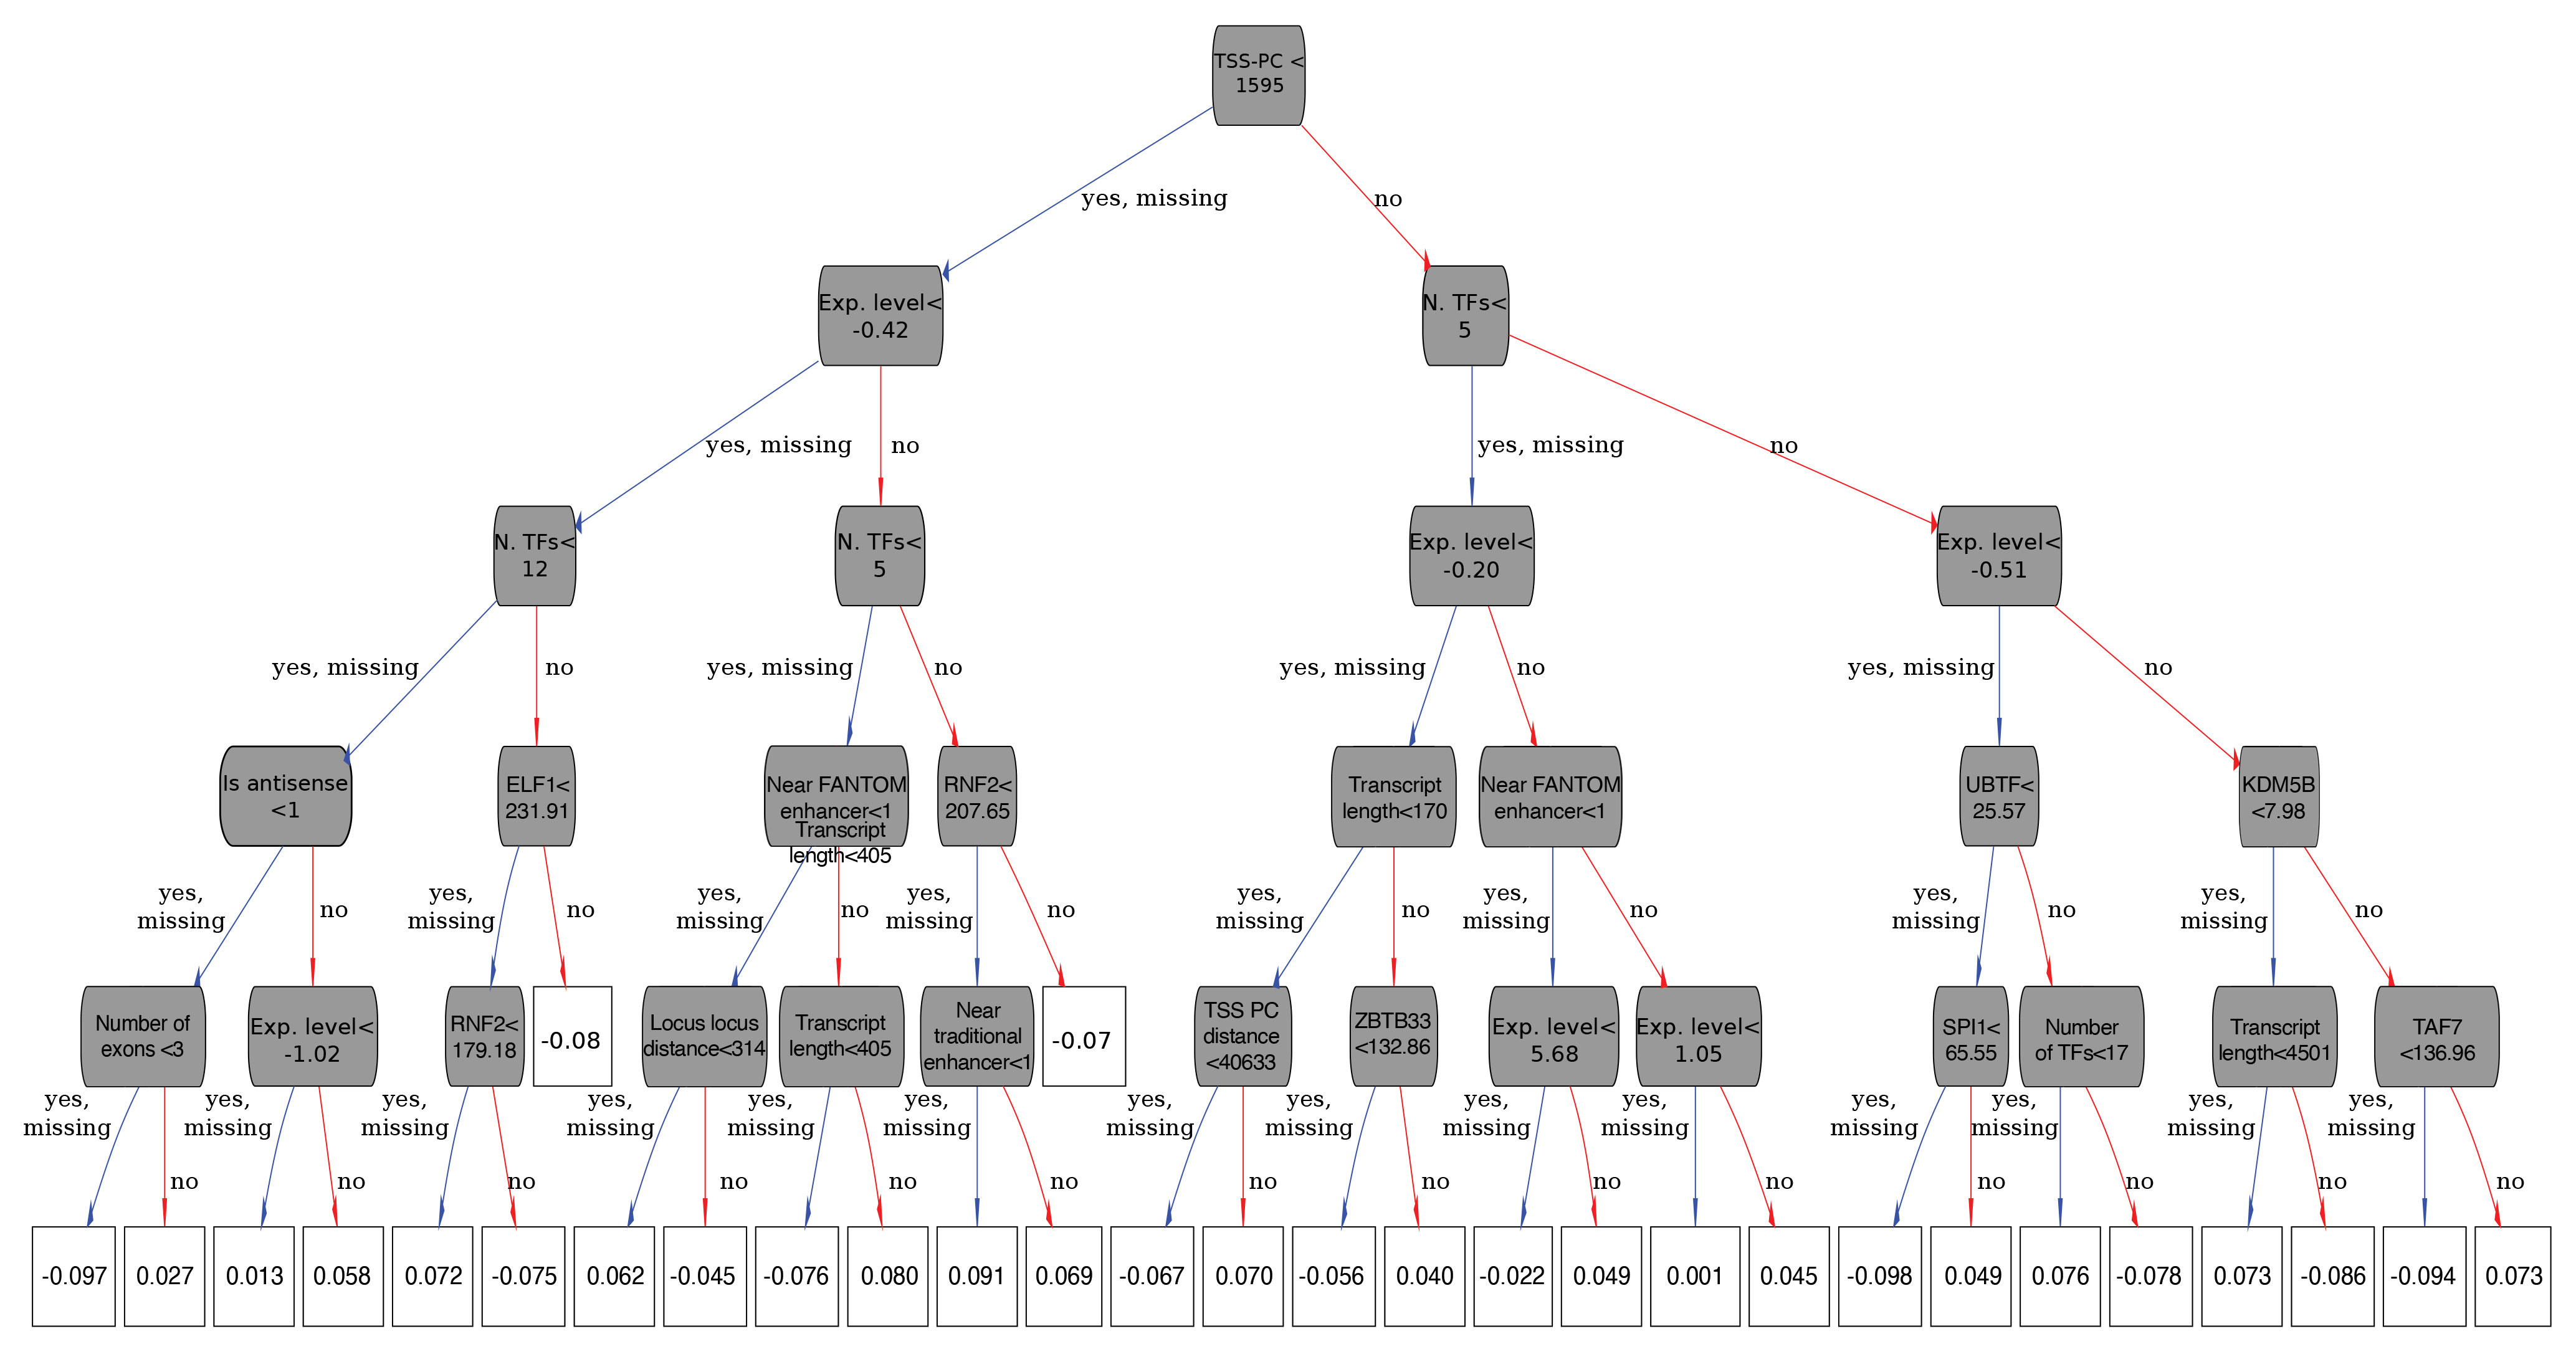
\includegraphics[width=0.95\textwidth]{plots/appendix/ml/first.residual.tree.png}
  \caption[XGBoost first residual-tree]{\textbf{XGBoost first residual-tree}. Tree nodes are represented as rounded grey boxes, and squared white boxes are the tree leafs.}
  \label{supp-fig:decision-tree}
\end{figure}

\begin{figure}[ht!]
  \centering
  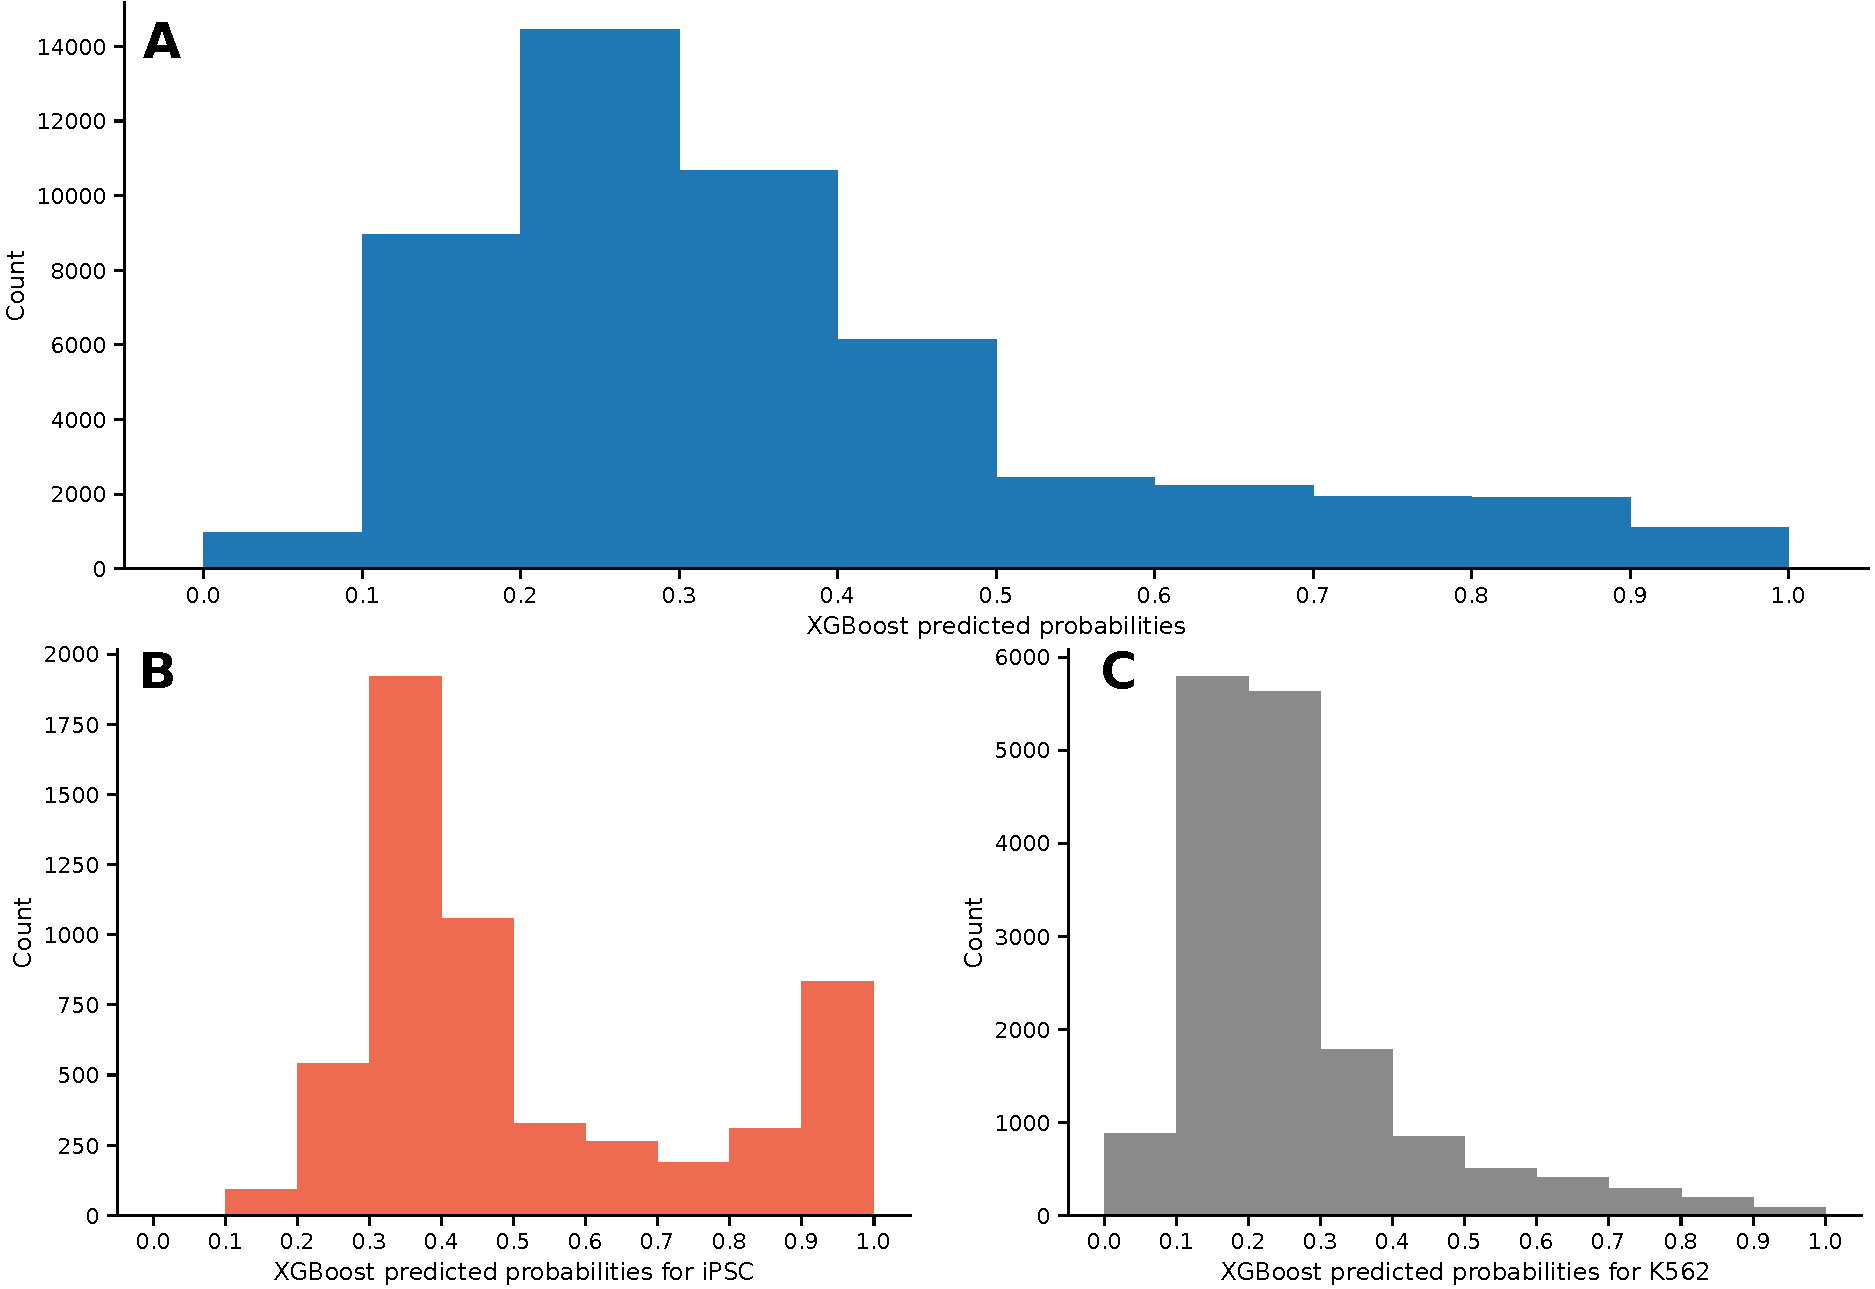
\includegraphics[scale=0.4]{plots/appendix/ml/xgboost.predict.prob.pdf}
  \caption[XGBoost predicted probabilities]{\textbf{XGBoost predicted probabilities}. \textbf{(A)} Probability distribution aggregated across the 7 cell types. \textbf{(B)} iPSC probabilities. \textbf{(C)} K562 probabilities.}
  \label{supp-fig:xgb-prob}
\end{figure}

\begin{figure}[ht!]
  \centering
  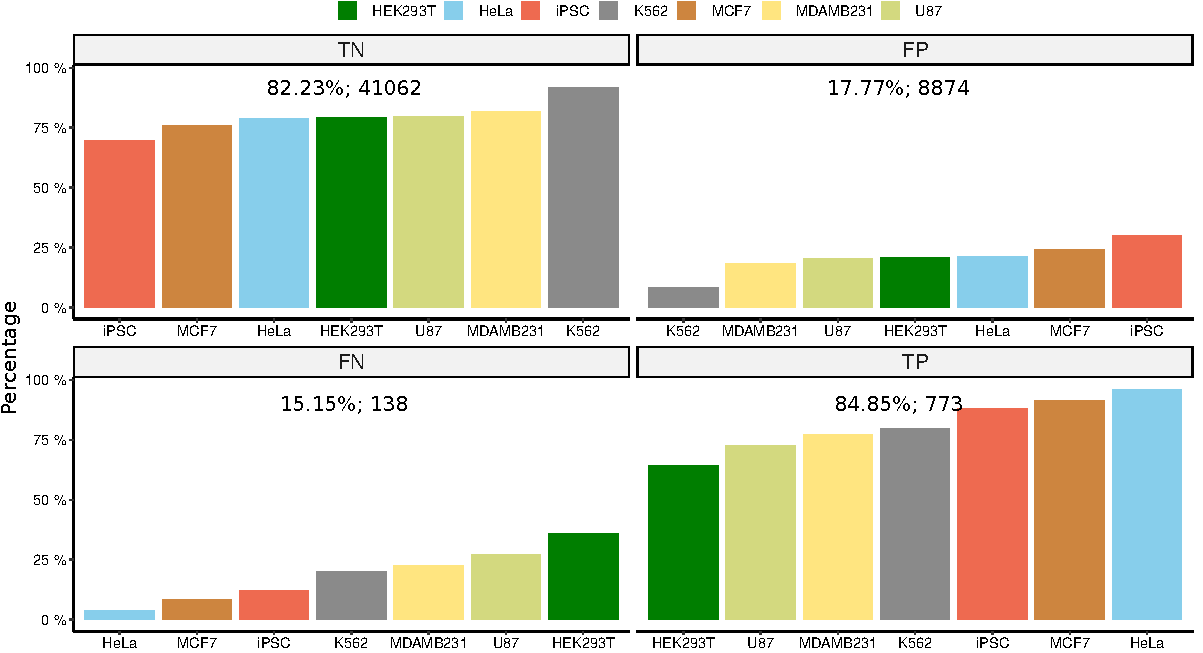
\includegraphics[scale=0.65]{plots/appendix/ml/cm.for.cell.pdf}
  \caption[Cell-type confusion matrix]{\textbf{Cell-type confusion matrix}. Confusion matrix based on model prediction for each cell line. Bar plots are sorted by percentage.}
  \label{supp-fig:cm-cell}
\end{figure}

\begin{figure}[!htb]
  \centering
  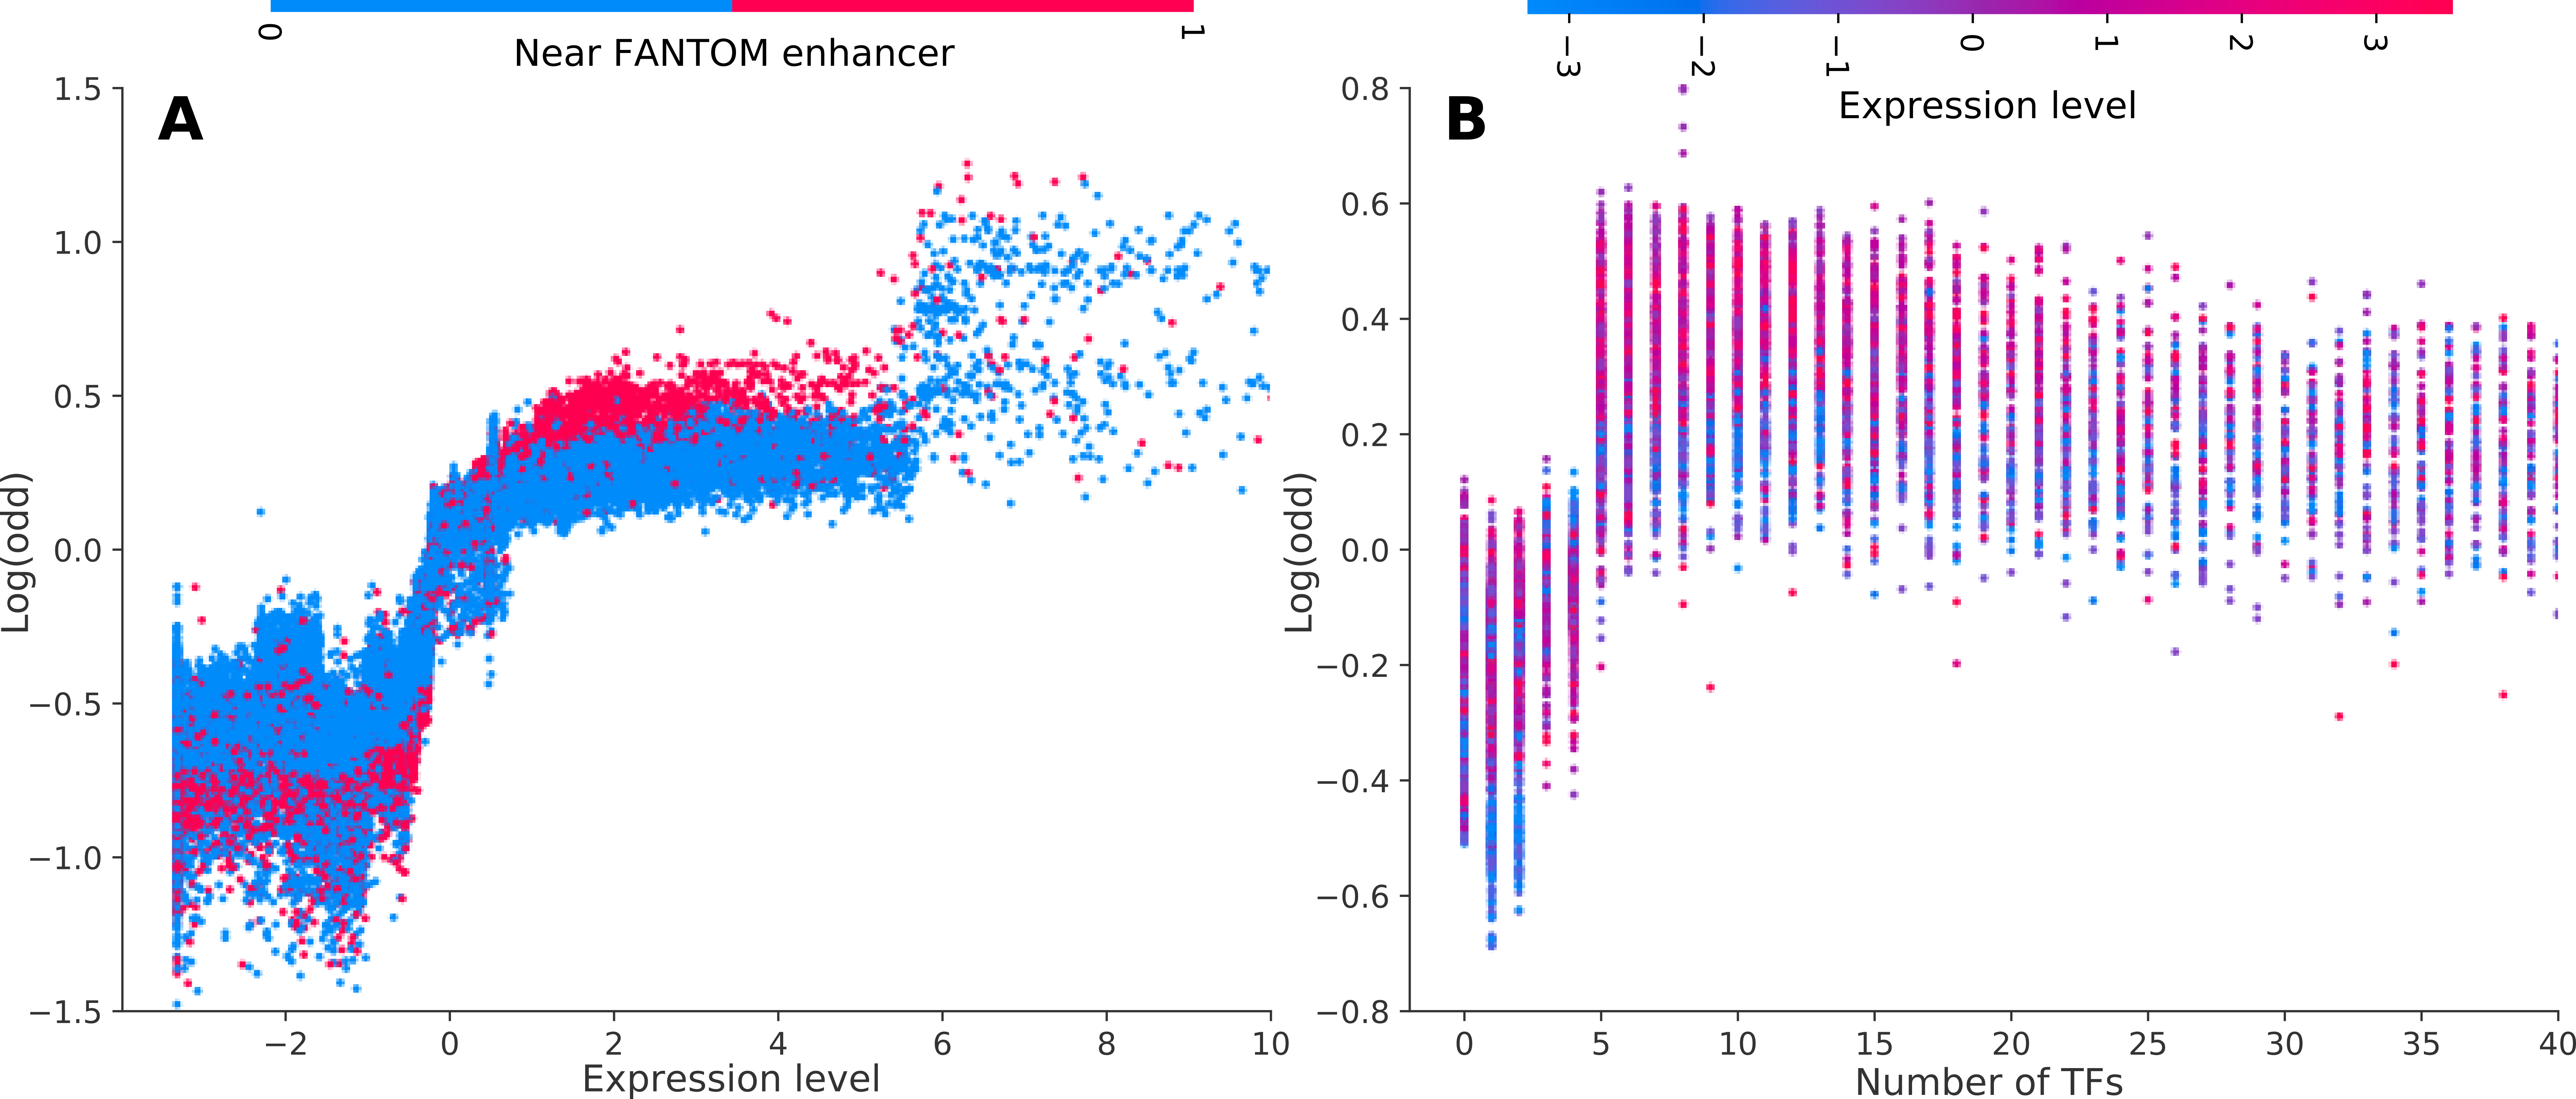
\includegraphics[width=0.9\textwidth]{plots/appendix/ml/shap.dep.interactions.png}
  \caption[SHAP dependence plots with interactions]{\textbf{SHAP dependence plots with interactions}. \textbf{(A)} Model explainability for lncRNA expression, blue dots represent lncRNAs whose transcript bodies reside not near from a FANTOM enhancer, and red dots near. \textbf{(B)} Dependence plot for number of TFs, each dot indicates a lncRNA loci with its associated expression value.}
  \label{supp-fig:shap-dep-interact}
\end{figure}

\begin{figure}[ht!]
  \centering
  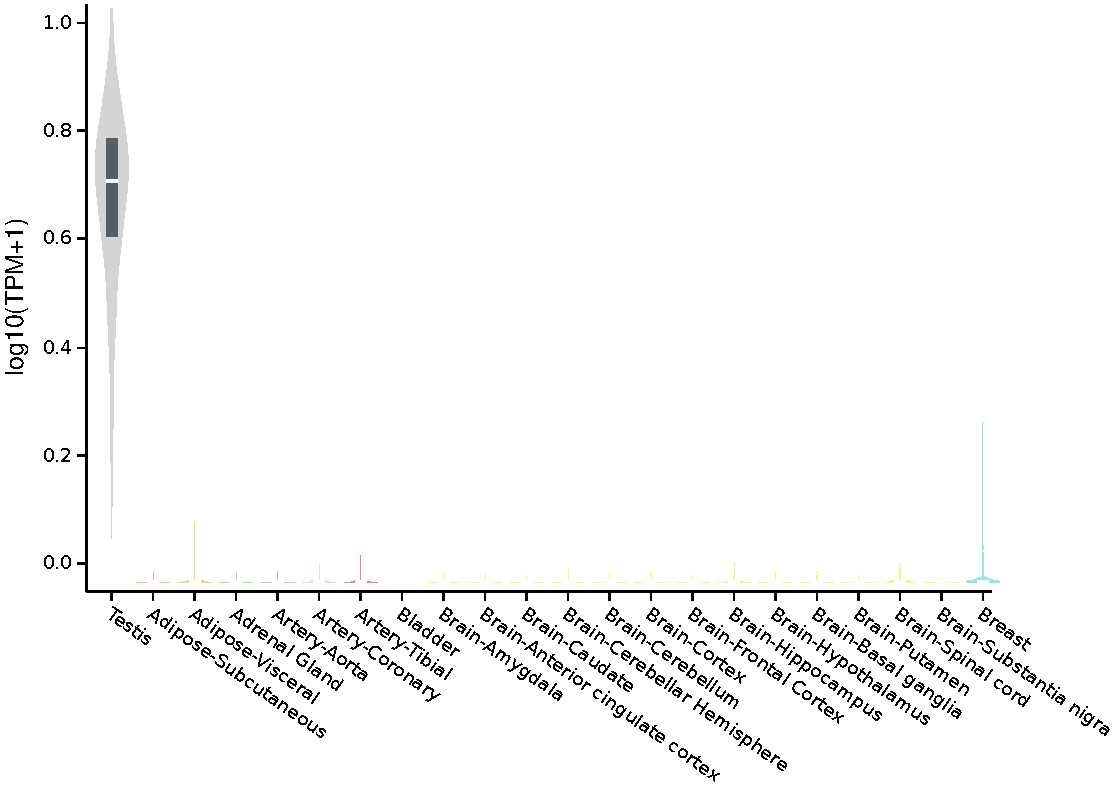
\includegraphics[scale=0.55]{plots/appendix/ml/linc00789.gene.expression.pdf}
  \caption[Tissue expression for \textit{LINC00879}]{\textbf{Tissue expression for \textit{LINC00879}}. Top 22 tissues with more gene expression and sorted by their medians. Expression values (log$_{10}$(TPM+1)) were based on GTEx v8.}
  \label{supp-fig:linc-gene-expression}
\end{figure}

\begin{figure}[ht!]
  \centering
  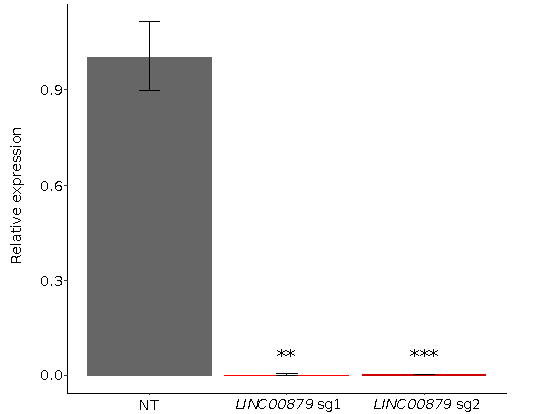
\includegraphics[scale=0.9]{plots/appendix/ml/qPCR.josh.results.pdf}
  \caption[\textit{LINC00879} qPCR]{\textbf{\textit{LINC00879} qPCR}. qPCR confirmation of \textit{LINC00879} knockdown in K562 cell. NT= non-targeting sgRNA.}
  \label{supp-fig:qpcr-kd-linc}
\end{figure}

\clearpage

\subsection{LncRNA analysis of the \textit{Drosophila} genome during regeneration}
\label{sec:sup_fig_part_1}

\begin{figure}[ht!]
  \centering
  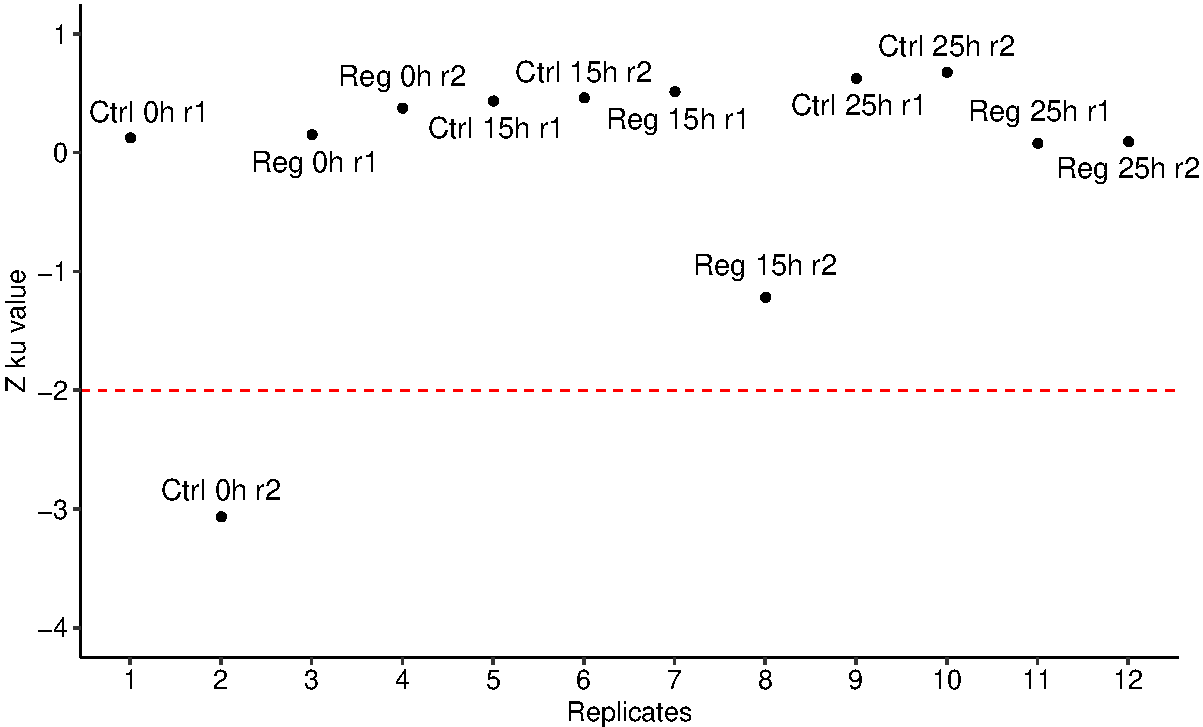
\includegraphics[scale=0.6]{plots/appendix/dme/connectivity.reg.pdf}
  \caption[WGCNA of regeneration data]{\textbf{WGCNA of regeneration data}. Horizontal dashed line highlights 2 standard deviations from a normal distribution. Ctrl= uninjured replicates; reg= injured; r= replicate.}
  \label{supp-fig:connectivity-reg}
\end{figure}

\begin{figure}[ht!]
  \centering
  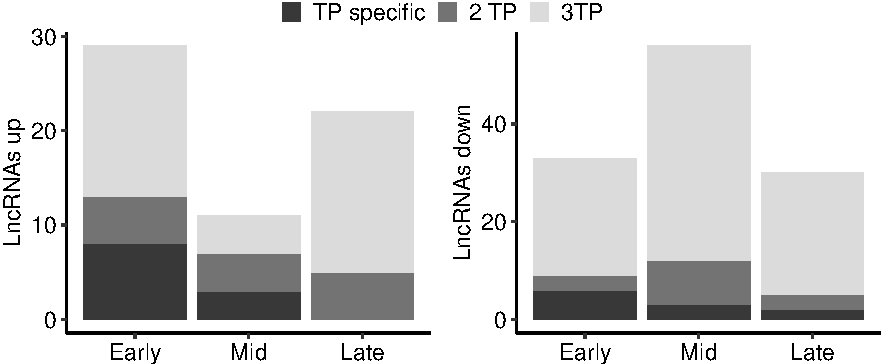
\includegraphics[scale=0.75]{plots/appendix/dme/time.point.specificity.pdf}
  \caption[Time-point specificity by DE status]{\textbf{Time-point specificity by DE status}. LncRNAs up and downregulated. TP specific= expressed only on the analyzed time-point; 2 TP and 3 TP expressed on 2 and 3 time-points, respectively.}
  \label{fig:time-point-specific-up-down}
\end{figure}

\begin{figure}[!htb]
  \centering
  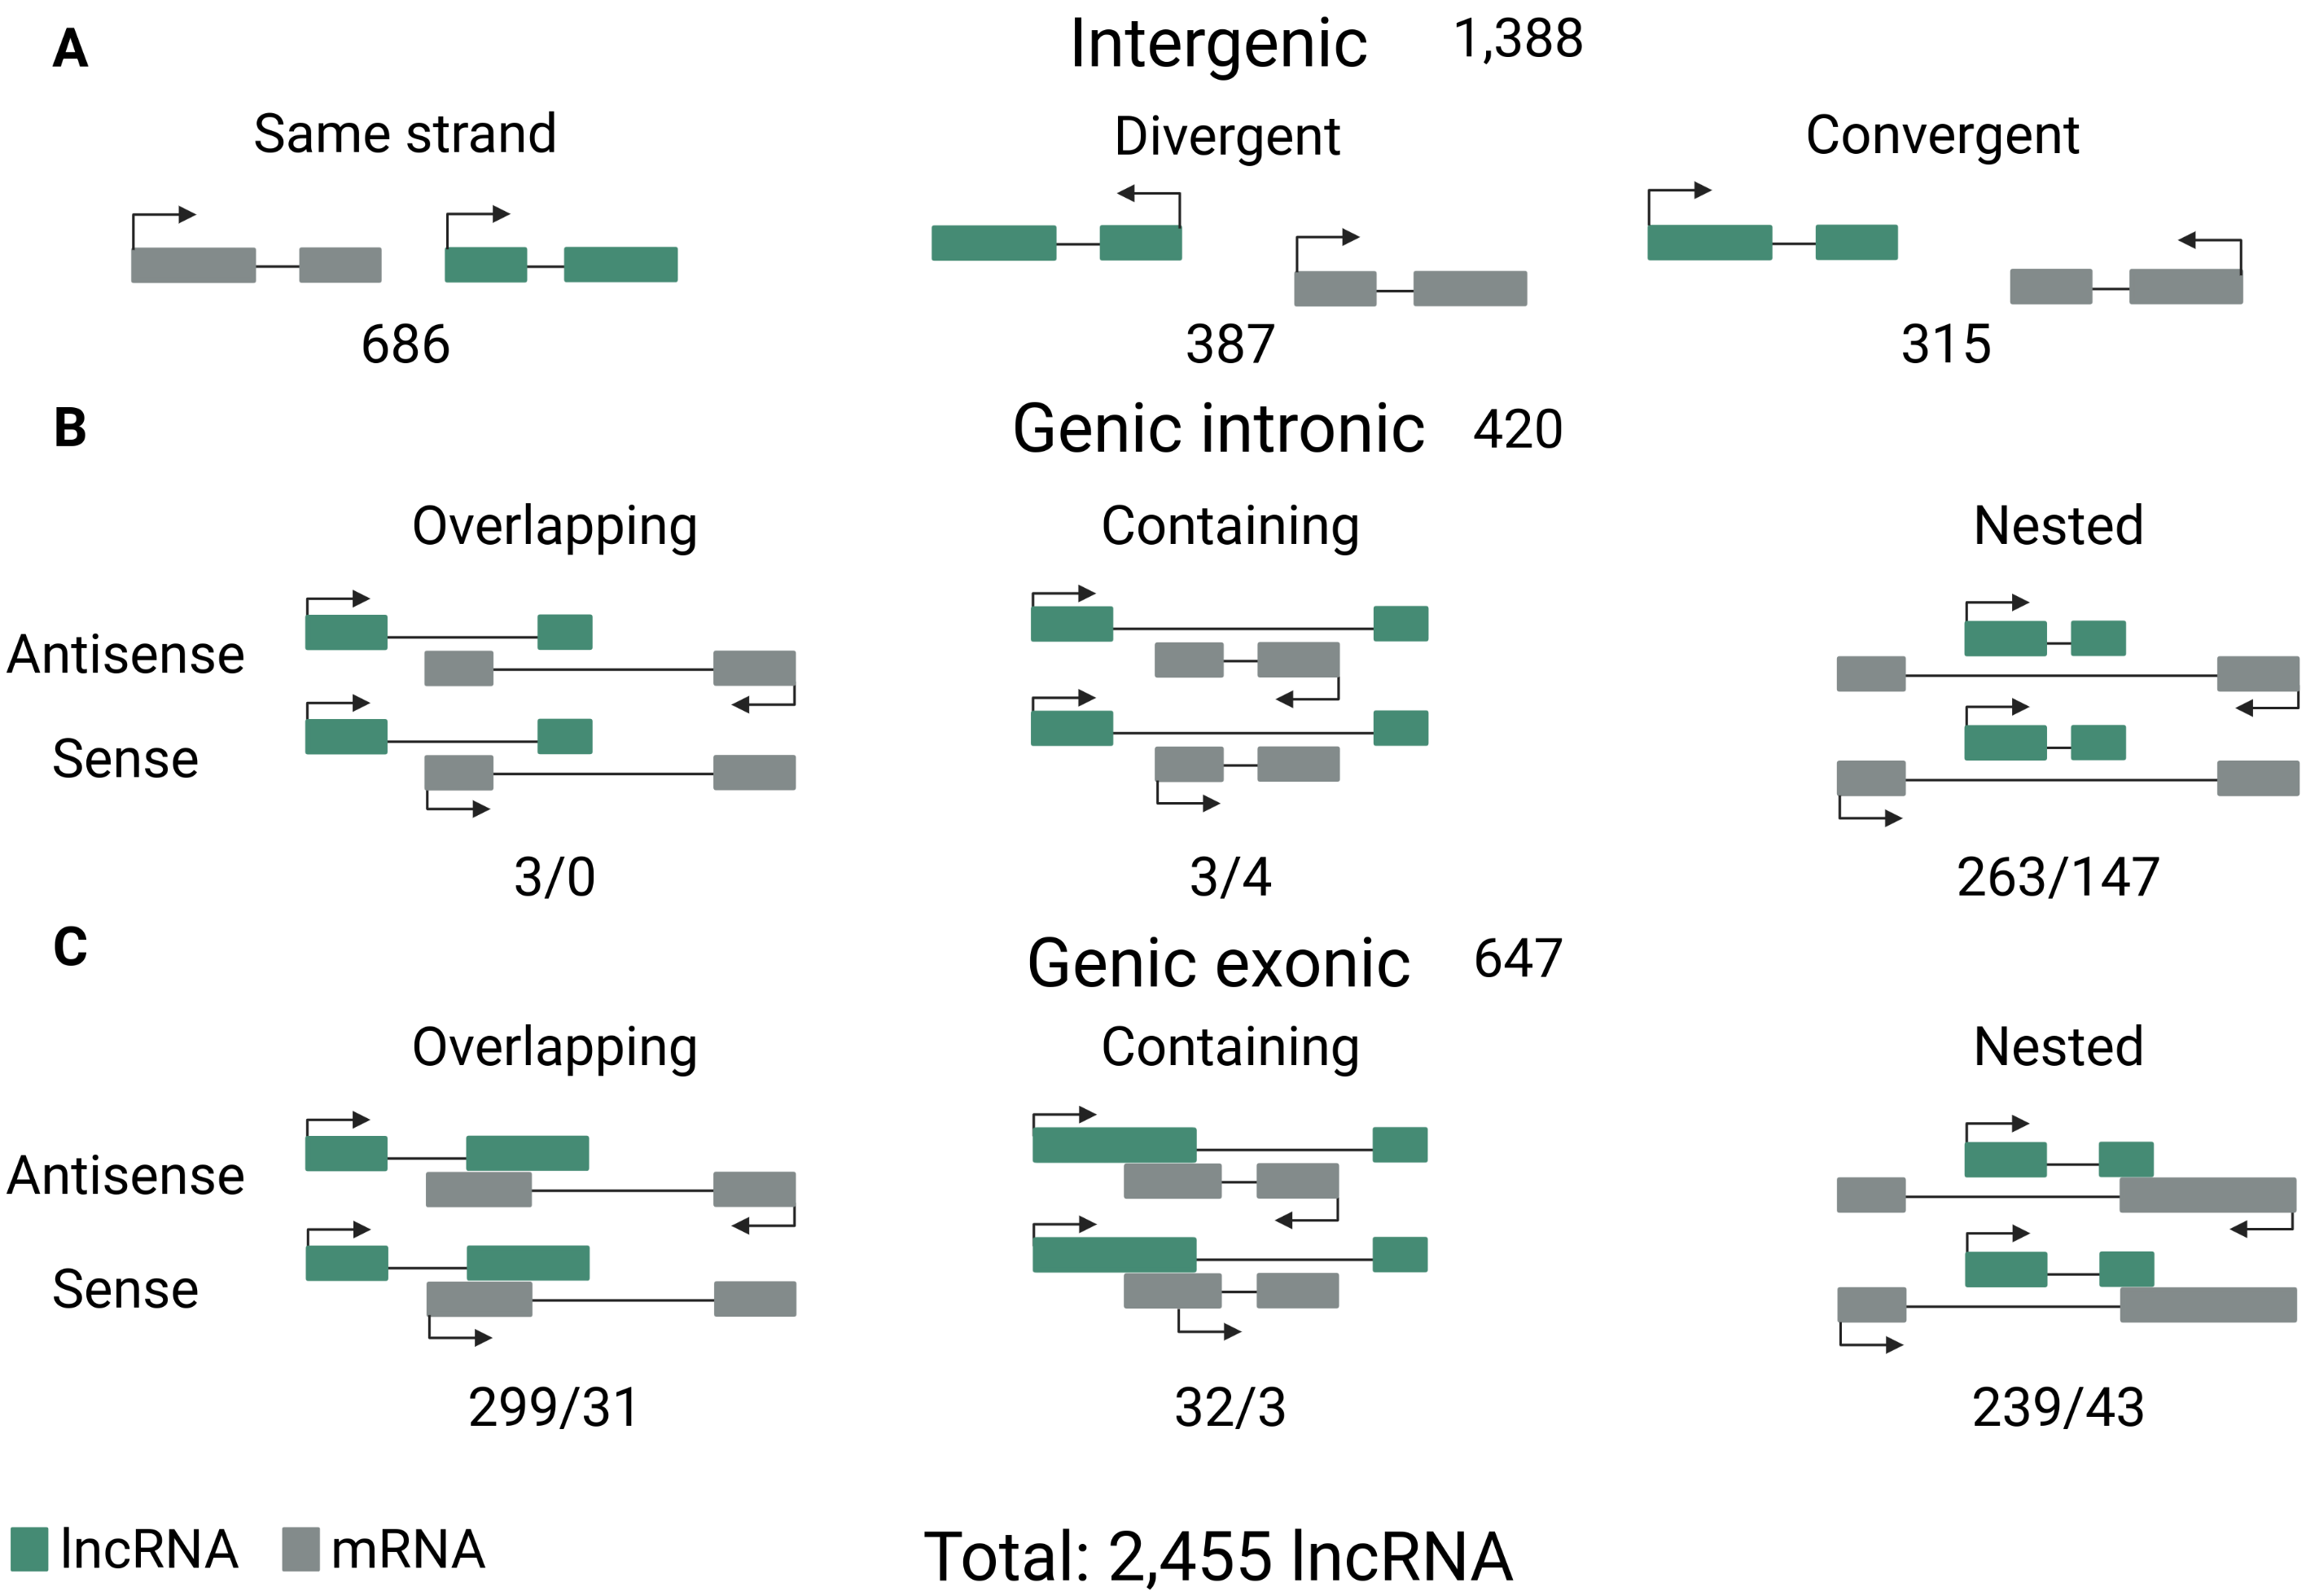
\includegraphics[width=0.8\textwidth]{img/appendix/dme/lncRNA_gw_classification.png}
  \caption[Genome-wide lncRNA classification]{\textbf{Genome-wide lncRNA classification}. \textbf{(A)} Intergenic classification. \textbf{(B,C)} Genic intronic and genic exonic, respectively. Numbers on the right represent the total for that classification, and numbers below show subclass frequencies. Nomenclature inspired by \autocite{wucher_2017}}
  \label{fig:gw_lncRNA_class}
\end{figure}

\begin{figure}[ht!]
  \centering
  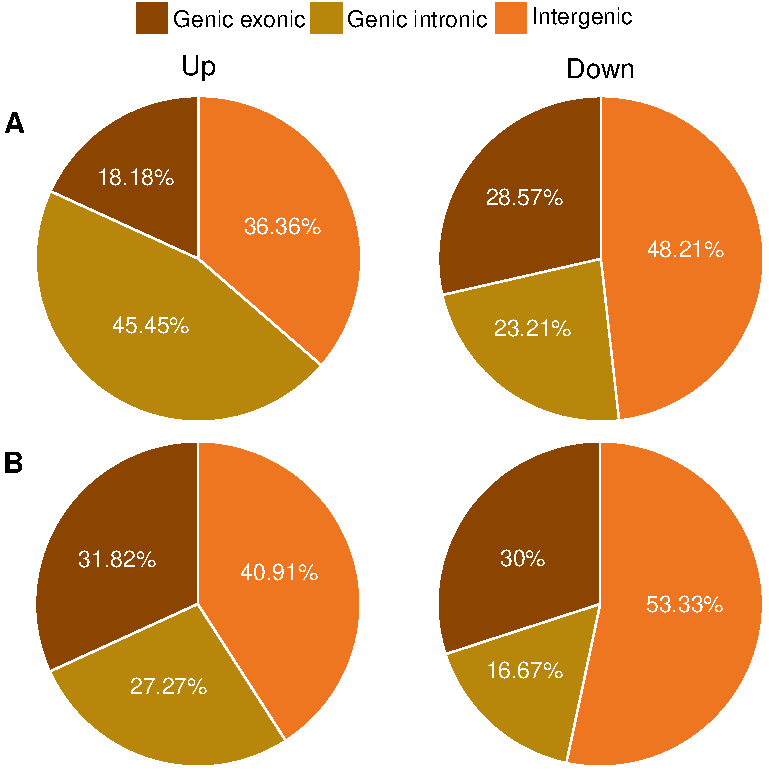
\includegraphics[scale=0.5]{plots/appendix/dme/lncRNA.class.mid.late.tp.pdf}
  \caption[Mid and late lncRNA classification]{\textbf{Mid and late lncRNA classification}. \textbf{(A)} LncRNA classification for genes up and downregulated at mid time-point. \textbf{(B)} Classification for late DEGs. }
  \label{supp-fig:mid-late-class}
\end{figure}

\begin{figure}[ht!]
  \centering
  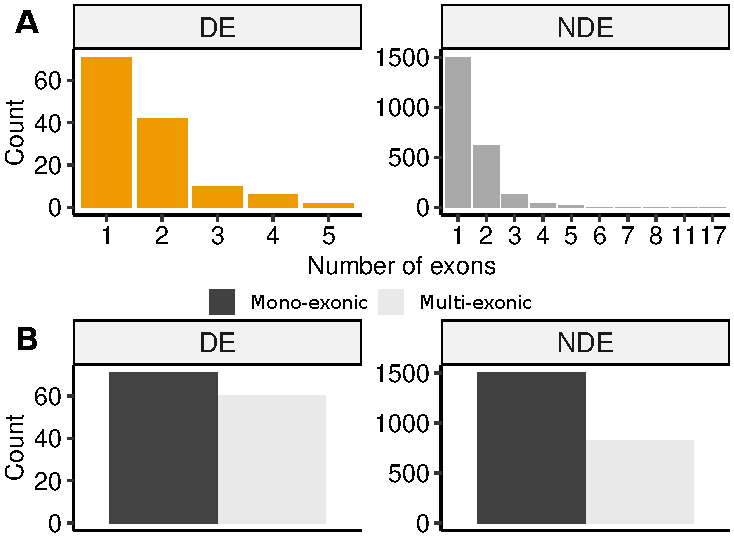
\includegraphics[scale=0.65]{plots/appendix/dme/number.exons.pdf}
  \caption[Number of exons]{\textbf{Number of exons}. \textbf{(A)} Number of exons of the 131 DE and not differentially expressed (NDE) lncRNAs. \textbf{(B)} Proportion of mono and multi-exonic transcripts. Analysis based on the longest transcript, multi-exonic $\ge$ 2 exons.}
  \label{supp-fig:number-exons}
\end{figure}

\begin{figure}[ht!]
  \centering
  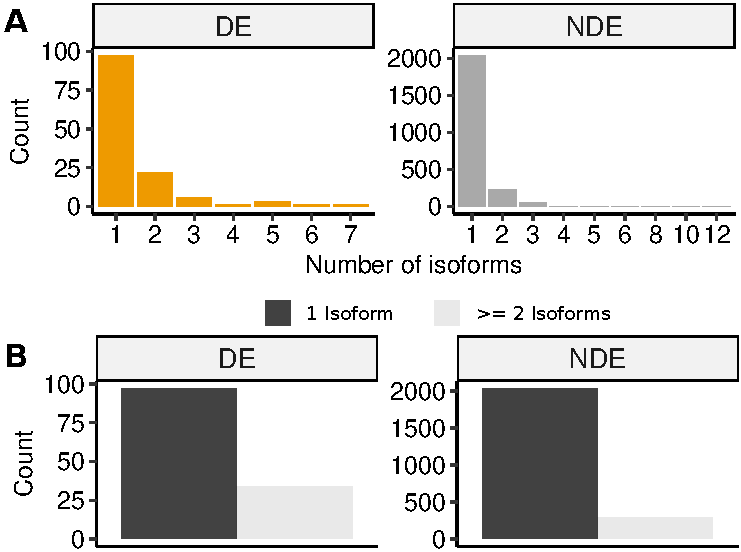
\includegraphics[scale=0.65]{plots/appendix/dme/isoform.analysis.pdf}
  \caption[Isoform analysis]{\textbf{Isoform analysis}. \textbf{(A)} Number of isoform comparison among the 131 DE and NDE lncRNAs. \textbf{(B)} Proportions of genes with one isoform and genes with $\ge$ 2 isoforms.}
  \label{supp-fig:isoform-analysis}
\end{figure}

\begin{figure}[ht!]
  \centering
  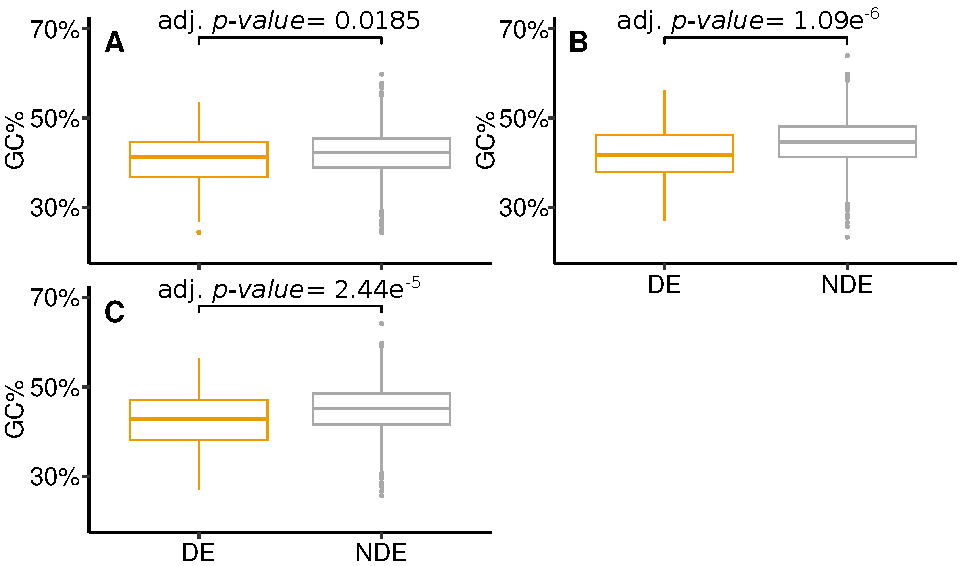
\includegraphics[scale=0.65]{plots/appendix/dme/gc.content.pdf}
  \caption[LncRNA GC content]{\textbf{LncRNA GC content}. \textbf{(A)} Promoter GC\%. \textbf{(B)} GC content of genes (\textit{i.e.} introns and exons). \textbf{(C)} GC\% based on the longest transcript.}
  \label{supp-fig:gc-content}
\end{figure}

\begin{figure}[ht!]
  \centering
  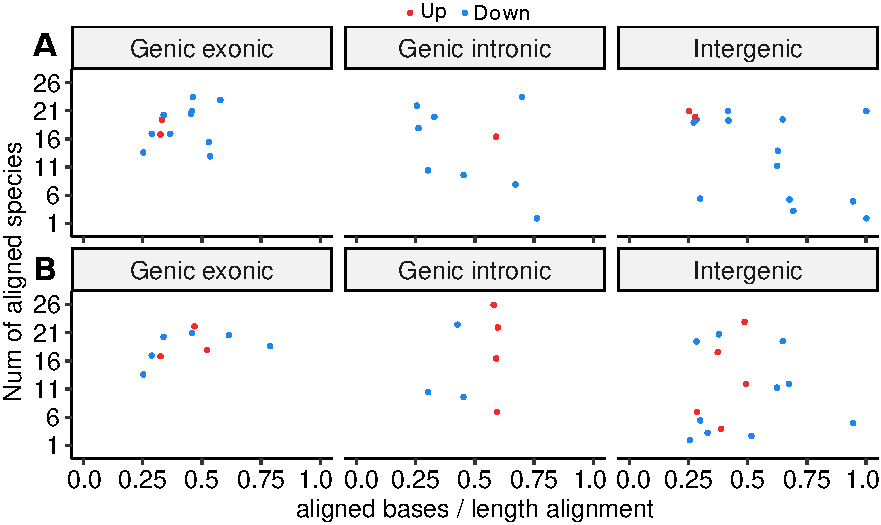
\includegraphics[scale=0.65]{plots/appendix/dme/seq.conservation.mid.late.pdf}
  \caption[Sequence conservation of mid and late lncRNAs]{\textbf{Sequence conservation of mid and late lncRNAs}. \textbf{(A,B)} DE lncRNAs at mid and late time-point, respectively.  Each dot represents a conserved lncRNA, and \textit{y-axis} shows the number of species that present the lncRNA conserved.}
  \label{supp-fig:lncRNA-seq-conservation}
\end{figure}

\begin{figure}[ht!]
  \centering
  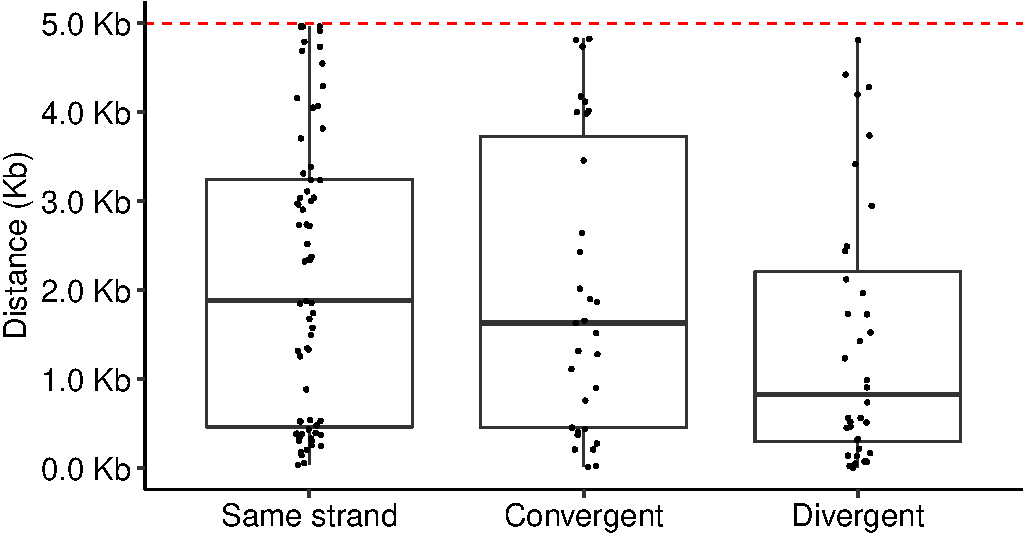
\includegraphics[scale=0.6]{plots/appendix/dme/linc.PCG.distance.pdf}
  \caption[LincRNA-PCG pairs distance]{\textbf{LincRNA-PCG pairs distance}. Intergenic subclassification boxplots sorted by higher to lower locus-locus distance. Dashed red line depicts the distance cutoff to assign a lincRNA-PCG pair.}
  \label{supp-fig:lincRNA-distance}
\end{figure}


\begin{figure}[ht!]
  \centering
  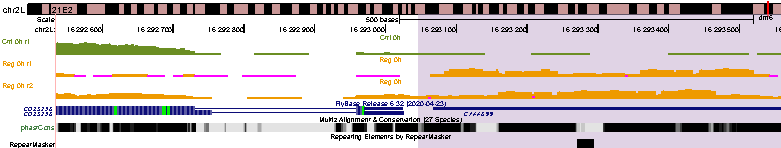
\includegraphics[width=1\textwidth]{plots/appendix/dme/cr44899.ucsc.plot.pdf}
  \caption[\textit{CR44899 UCSC} plot]{\textbf{\textit{CR44899 UCSC} plot}. RNA-seq data, gene structure, conservation, and repeats of \textit{CR44899} lncRNA. Blue boxes represent coding and noncoding genes. .}
  \label{supp-fig:cr43611-ucsc}
\end{figure}

\begin{figure}[ht!]
  \centering
  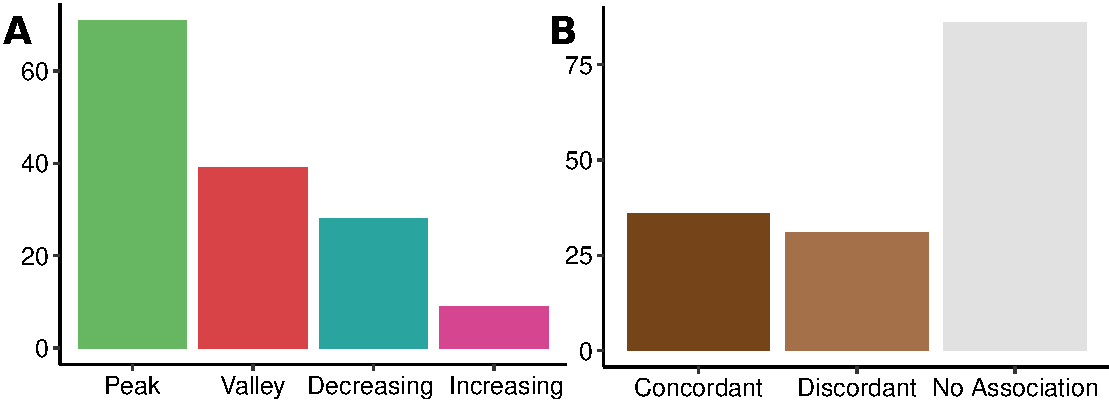
\includegraphics[scale=0.6]{plots/appendix/dme/co.expression.ctrl.pdf}
  \caption[Co-expression results in control]{\textbf{Co-expression results in control}. \textbf{(A)} Co-expression classification in control. \textbf{(B)} Co-expression results in control.}
  \label{supp-fig:co-exp-ctrl}
\end{figure}

\begin{figure}[ht!]
  \centering
  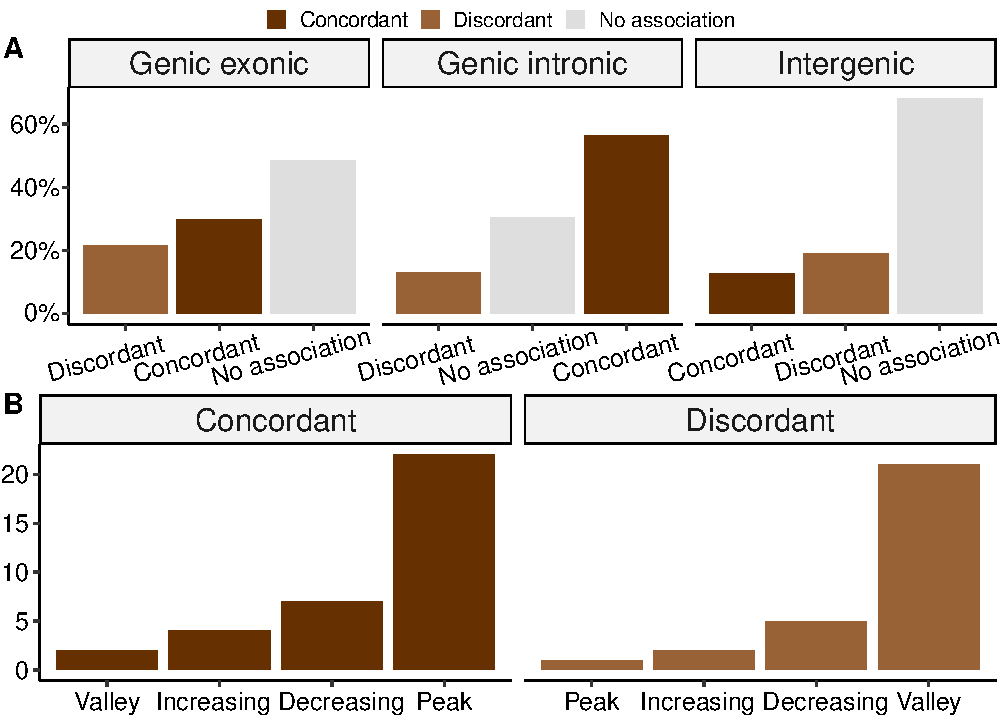
\includegraphics[scale=0.6]{plots/appendix/dme/co.expression.within.reg.pdf}
  \caption[Co-expression within regeneration]{\textbf{Co-expression within regeneration}. \textbf{(A)} Co-expression classification by lncRNA genomic position. \textbf{(B)} LncRNA defines co-expression classification labels for concordant and discordant cases.}
  \label{fig:co-exp-supp-fig}
\end{figure}

\begin{figure}[ht!]
  \centering
  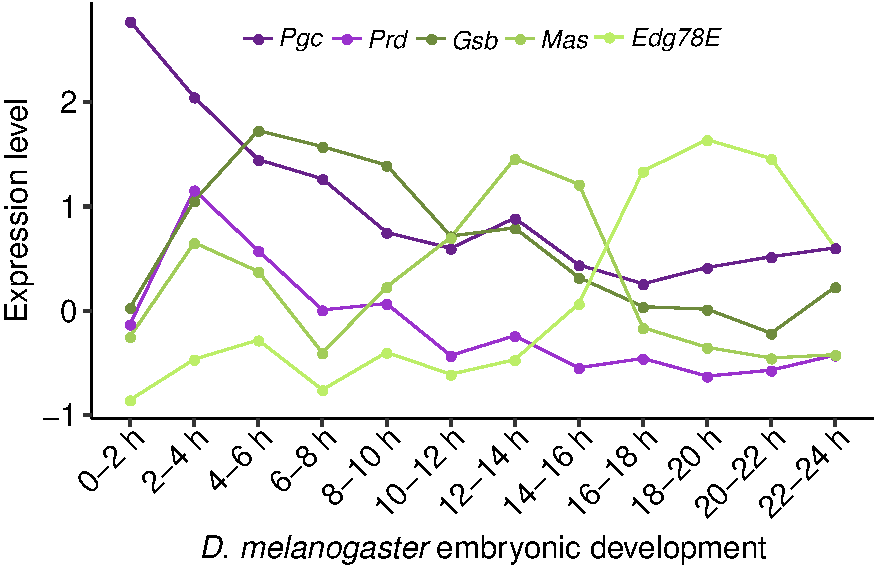
\includegraphics[scale=0.65]{plots/appendix/dme/markers.pdf}
  \caption[Developmental markers]{\textbf{Developmental markers}. Expression profiles in log$_{10}$(TPM+0.1) for five developmental marker genes.}
  \label{supp-fig:markers-dev}
\end{figure}

\begin{figure}[ht!]
  \centering
  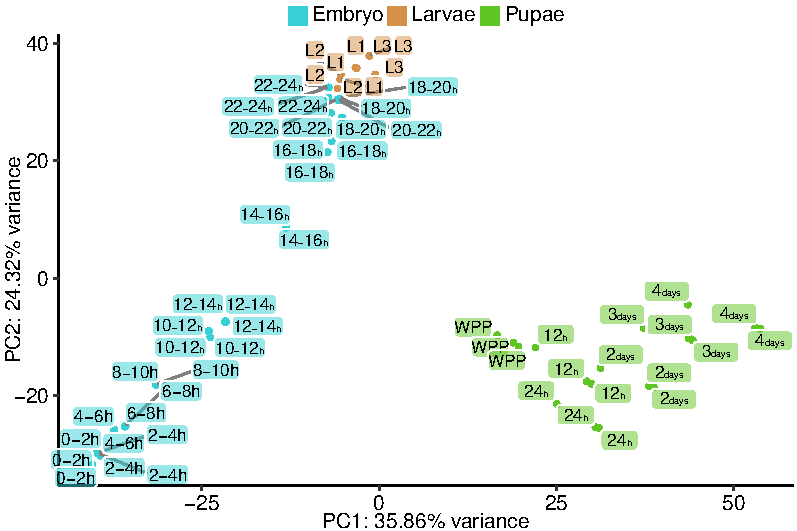
\includegraphics[scale=0.7]{plots/appendix/dme/modencode.pca.pdf}
  \caption[PCA of developmental samples]{\textbf{PCA of developmental samples}. PCA based on expressed genes, coding and noncoding, in log$_{10}$(TPM+0.1) within the developmental dataset.}
  \label{supp-fig:pca-modencode}
\end{figure}

\begin{figure}[ht!]
  \centering
  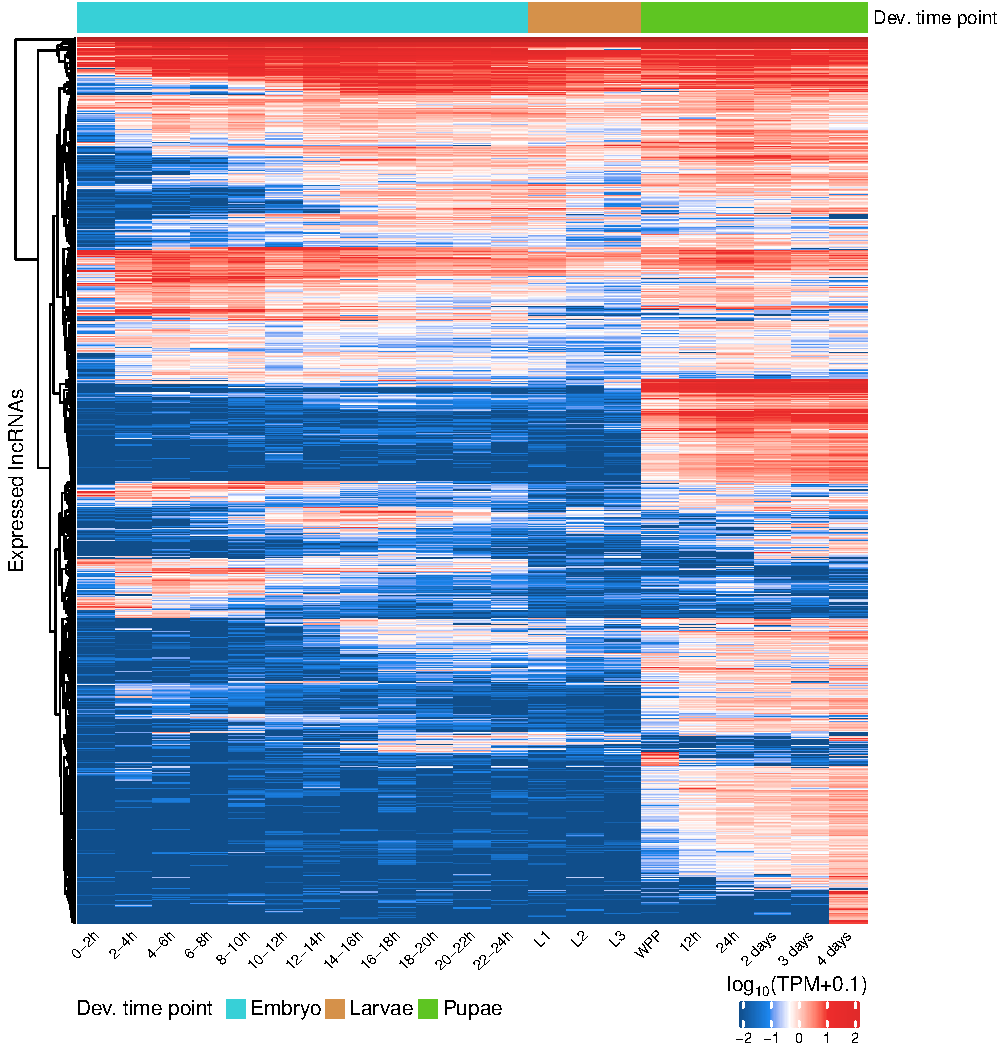
\includegraphics[scale=0.5]{plots/appendix/dme/all.lncRNA.exp.dev.pdf}
  \caption[Developmental profile of lncRNAs]{\textbf{Developmental profile of lncRNAs}. LnRNAs (rows) expressed across development (columns) from 0h-2h embryo to 4 days pupae.}
  \label{fig:heatmap-modencode-dev-all}
\end{figure}

\begin{figure}[ht!]
  \centering
  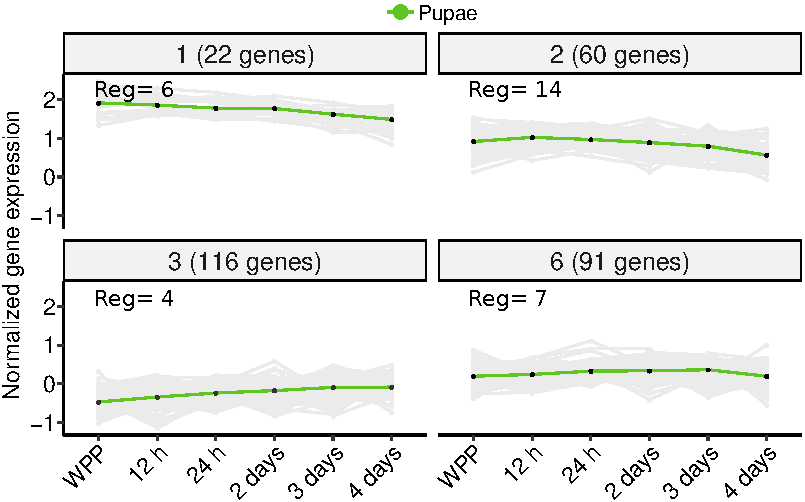
\includegraphics[scale=0.75]{plots/appendix/dme/puape.supp.clusters.pdf}
  \caption[Pupal developmental clusters]{\textbf{Pupal developmental clusters}. K-means clustering based on pupal developmental expression. \textit{Y-axis} shows the normalized and scaled gene expression levels.}
  \label{supp-fig:pupae-clustering}
\end{figure}

\begin{figure}[ht!]
  \centering
  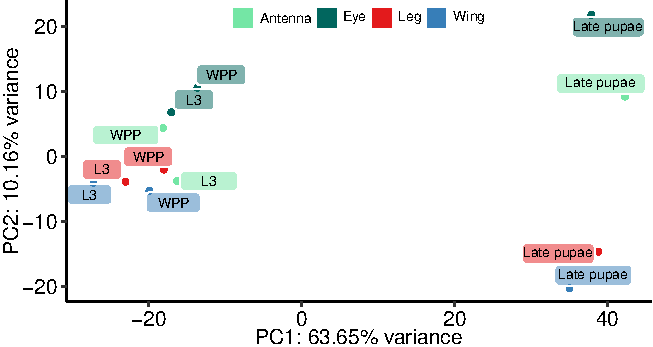
\includegraphics[scale=0.9]{plots/appendix/dme/erc.pca.pdf}
  \caption[PCA of imaginal discs]{\textbf{PCA of imaginal discs}. PCA based on expressed genes, coding and noncoding, in log$_{10}$(TPM+0.1) within the antenna, eye, leg, and wing imaginal disc data.}
  \label{supp-fig:pca-erc}
\end{figure}

\begin{figure}[ht!]
  \centering
  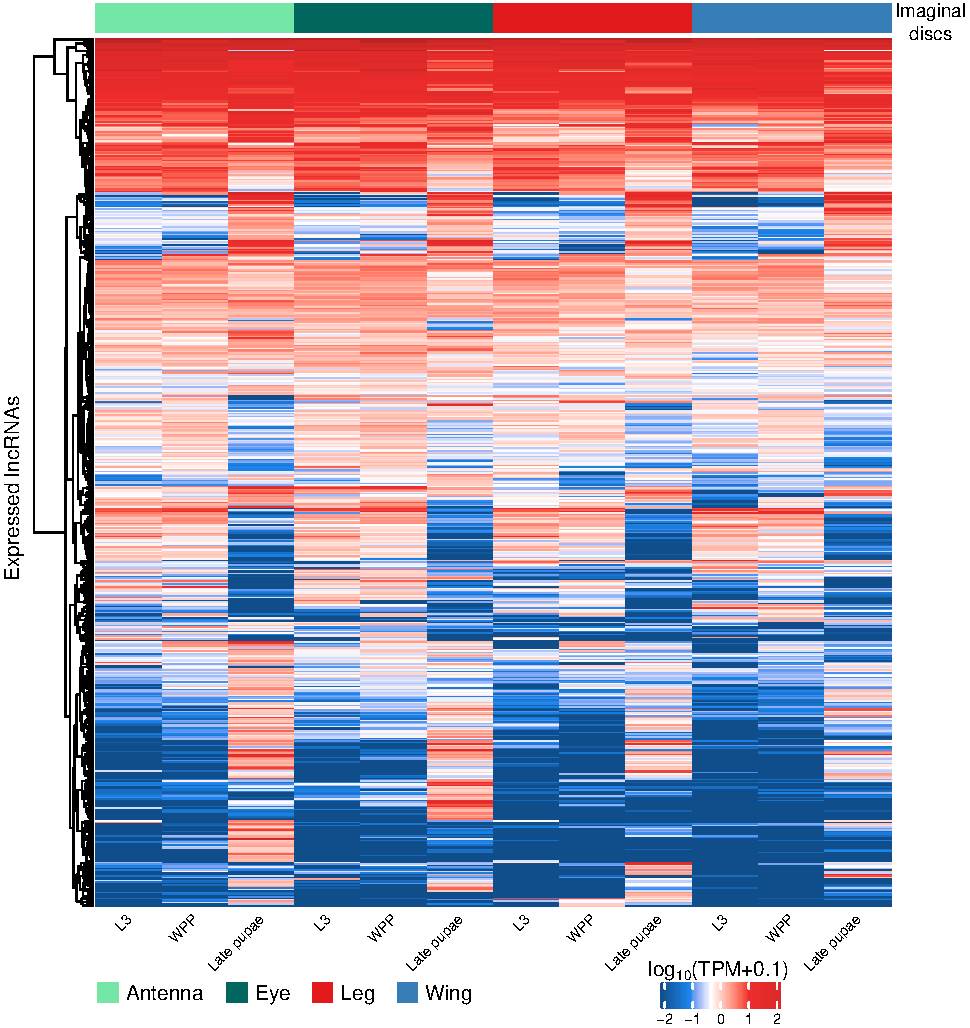
\includegraphics[scale=0.7]{plots/appendix/dme/all.lncRNA.exp.erc.pdf}
  \caption[Imaginal disc profile of lncRNAs]{\textbf{Imaginal disc profile of lncRNAs}. LncRNAs (rows) expressed across antenna, eye, leg and wing imaginal discs (columns) in three developmental time points: L3, WPP, and late pupae. Samples are sorted by developmental time point.}
  \label{fig:heatmap-erc-all}
\end{figure}

\begin{figure}[ht!]
  \centering
  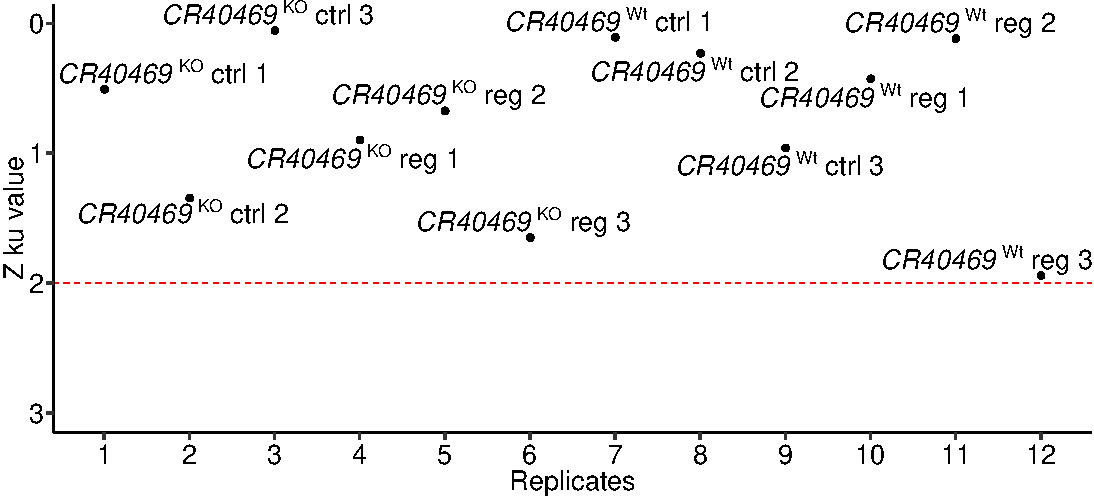
\includegraphics[scale=0.6]{plots/appendix/dme/cr40469.ko.wgcna.pdf}
  \caption[WGCNA of \textit{CR40469} KO replicates]{\textbf{WGCNA of \textit{CR40469} KO replicates}. Horizontal dashed line highlights 2 standard deviations from a normal distribution. Ctrl= uninjured replicates; reg= injured.}
  \label{supp-fig:wgcna-cr40469}
\end{figure}

\begin{figure}[ht!]
  \centering
  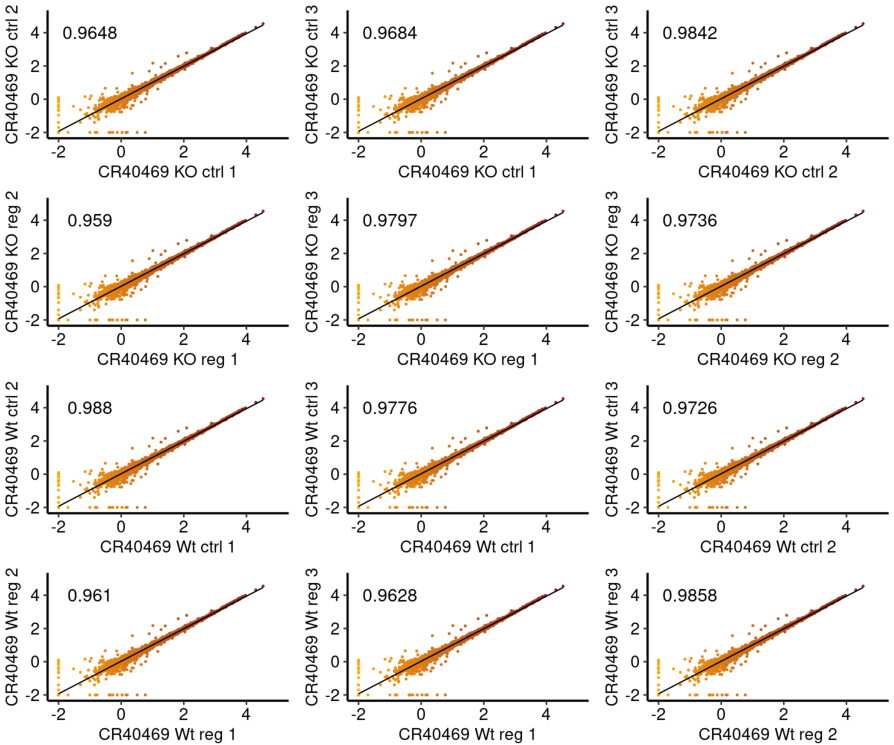
\includegraphics[scale=0.7]{plots/appendix/dme/qc.cr40469.pdf}
  \caption[Correlation of \textit{CR40469} KO replicates]{\textbf{Correlation of \textit{CR40469} KO replicates}. Pearson correlation among RNA-seq replicates.}
  \label{fig:qc-cr404-rna-seq}
\end{figure}

\begin{figure}[ht!]
  \centering
  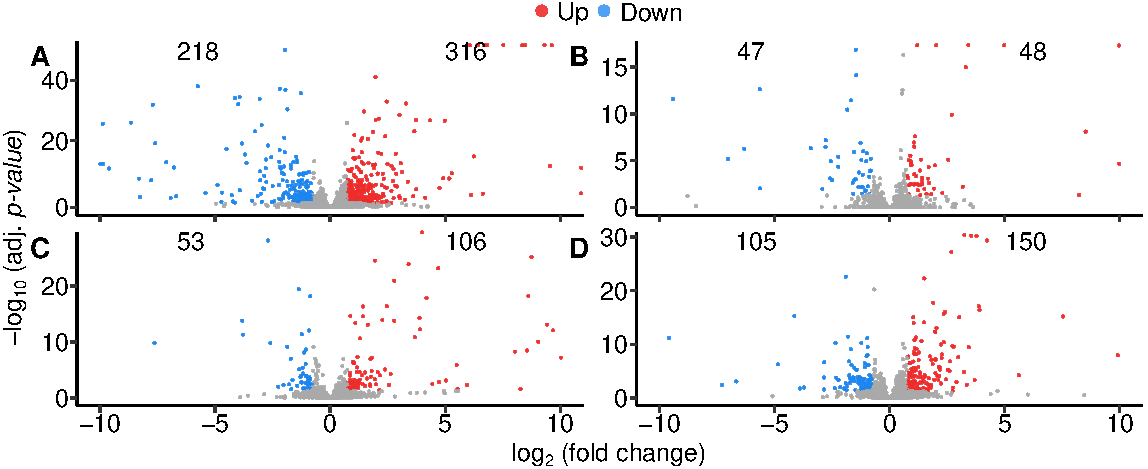
\includegraphics[scale=0.65]{plots/results/dme/volcano.plots.pdf}
  \caption[DE results of \textit{CR40469} KO]{\textbf{DE results of \textit{CR40469} KO}. \textbf{(A)} \textit{CR40469}$^{KO}$ vs. \textit{CR40469}$^{Wt}$ in control at 0h. \textbf{(B)} \textit{CR40469}$^{KO}$ vs. \textit{CR40469}$^{Wt}$ in regeneration at 0h. \textbf{(C)} Regeneration vs. control at 0h with \textit{CR40469}$^{KO}$. \textbf{(D)} Regeneration vs. control at 0h with \textit{CR40469}$^{Wt}$. Left and right numbers show down and up genes, respectively.}
  \label{fig:cr40469-volcano-plots}
\end{figure}

\begin{figure}[ht!]
  \centering
  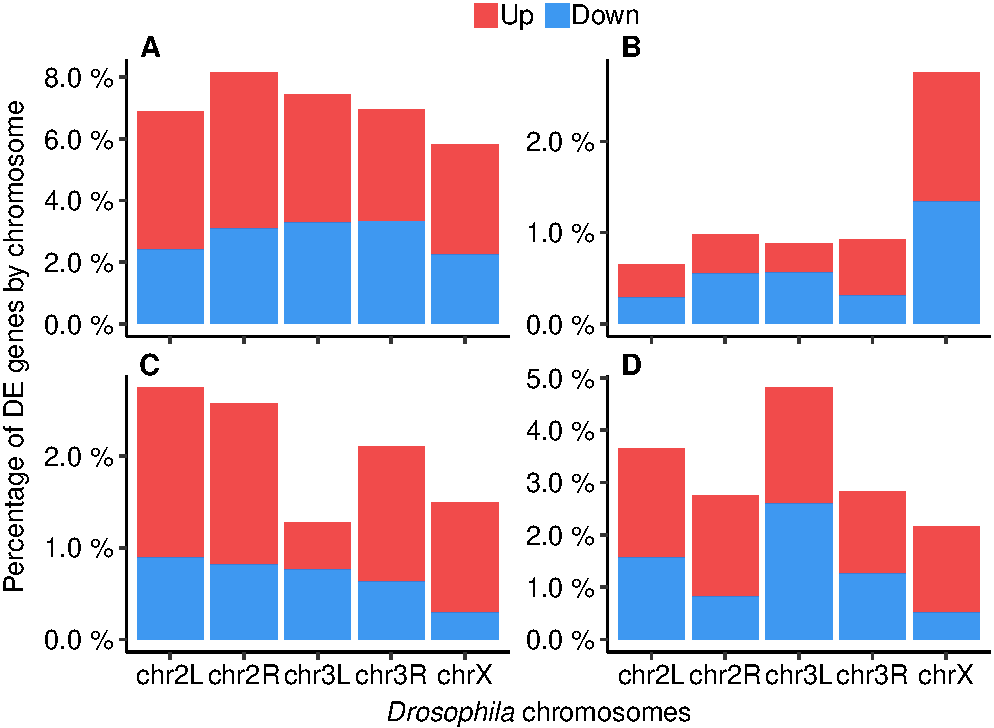
\includegraphics[scale=0.5]{plots/appendix/dme/cis.acting.cr40469.pdf}
  \caption[Distribution of DEGs by chromosome]{\textbf{Distribution of DEGs by chromosome}.  \textit{X-axis} shows the fruit fly chromosomes where DEGs were observed. Percentage  was calculated based on the number of DEGs by each chromosome divided by the number of expressed genes. Red and blue bars denote up and downregulated genes, respectively; for the following 4 combinations: \textbf{(A)} \textit{CR40469}$^{KO}$ vs. \textit{CR40469}$^{Wt}$ in control at 0h. \textbf{(B)} \textit{CR40469}$^{KO}$ vs. \textit{CR40469}$^{Wt}$ in regeneration at 0h. \textbf{(C)} Regeneration vs. control at 0h with \textit{CR40469}$^{KO}$. \textbf{(D)} Regeneration vs. control at 0h with \textit{CR40469}$^{Wt}$.}
  \label{supp-fig:cr40469-cis-acting}
\end{figure}

\clearpage

\section[Supplementary tables]{Supplementary tables}
\label{sec:supp_tables}

\subsection{XGBoost classifier to uncover the function of lncRNAs in cell-growth}
\label{sec:sup_tables_part_2}

\begin{table}[!htb]
  \caption[Cost-sensitive model metrics]{\textbf{Cost-sensitive model metrics}. Values based on the mean of 3 randomization seeds of the test set.}
  \begin{scriptsize}
    \begin{tabulary}{0.95\linewidth}{ccccccc}
      \textbf{Model} & \textbf{Sensitivity} & \textbf{Specificity} & \textbf{AUROC} & \textbf{F1}  & \textbf{Precision} & \textbf{Brier score}\\ \hline
      XGBoost & 0.7245 & 0.8224 & 0.8236 & 0.1264 & 0.0693 & 0.1638 \\
      Balanced random forest & 0.7603 & 0.8084 & 0.8335 & 0.1240 & 0.0675 & 0.1460 \\
      Logistic regression & 0.6165 & 0.8569 & 0.7788 & 0.1304 & 0.0629 & 0.1442 \\
    \end{tabulary}
  \end{scriptsize}
  \label{tab:summary_cost-sensitive_models}
\end{table}

\begin{table}[!htb]
  \caption[Under-sampling strategies without replacement]{\textbf{Under-sampling strategies without replacement}. Preprocessing sampling strategies applied before XGBoost training.}
  \begin{scriptsize}
    \begin{tabulary}{0.95\linewidth}{ccccccc}
      \multicolumn{6}{c}{ \textbf{Without replacement}} \\
      \textbf{Sampling strategy} & \textbf{Sensitivity} & \textbf{Specificity} & \textbf{AUROC} & \textbf{F1}  & \textbf{Precision}\\ \hline
      3\% & 0.1627 & 0.9961 & 0.8250 & 0.2360 & 0.4363 \\
      4\% & 0.2001 & 0.9942 & 0.8270 & 0.2621 & 0.3868  \\
      5\% & 0.2341 & 0.9924 & 0.8281 & 0.2818 & 0.3583 \\
      10\% & 0.3556 & 0.9826 & 0.8270 & 0.3073 & 0.2716 \\
      20\% & 0.4946 & 0.9588 & 0.8292 & 0.2633 & 0.1797 \\
      30\% & 0.5638 & 0.9342 & 0.8302 & 0.2182 & 0.1354 \\
      40\% & 0.6114 & 0.9111 & 0.8289 & 0.1888 & 0.1117 \\
      50\% & 0.6458 & 0.8894 & 0.8269 & 0.1679 & 0.0966 \\
    \end{tabulary}
  \end{scriptsize}
  \label{supp-tab:under-sampling-without-replacement}
\end{table}

\begin{table}[!htb]
  \caption[Under-sampling strategies with replacement]{\textbf{Under-sampling strategies with replacement}. Preprocessing sampling strategies applied before XGBoost training.}
  \begin{scriptsize}
    \begin{tabulary}{0.95\linewidth}{ccccccc}
      \multicolumn{6}{c}{ \textbf{With replacement}} \\
      \textbf{Sampling strategy} & \textbf{Sensitivity} & \textbf{Specificity} & \textbf{AUROC} & \textbf{F1}  & \textbf{Precision}\\ \hline
      3\% & 0.1895 & 0.9945 & 0.8238 & 0.2531 & 0.3858 \\
      4\% & 0.2301 & 0.9928 & 0.8257 & 0.2815 & 0.3665 \\
      5\% & 0.2594 & 0.9906 & 0.8258 & 0.2918 & 0.3356 \\
      10\% & 0.3604 & 0.9807 & 0.8307 & 0.2980 & 0.2546 \\
      20\% & 0.4873 & 0.9589 & 0.8316 & 0.2609 & 0.1784 \\
      30\% & 0.5675 & 0.9337 & 0.8301 & 0.2183 & 0.1353 \\
      40\% & 0.6172 & 0.918 & 0.8306 & 0.1915 & 0.1134 \\
      50\% & 0.6312 & 0.8897 & 0.8253 & 0.1646 & 0.0947 \\
    \end{tabulary}
  \end{scriptsize}
  \label{supp-tab:under-sampling-with-replacement}
\end{table}

\begin{table}[!htb]
  \caption[Features without predictive value]{\textbf{Features without predictive value}. Features with zero SHAP values.}
  \begin{scriptsize}
    \begin{tabulary}{0.95\linewidth}{ccccccc}
      Near VISTA enhancer & Locus is homozygous deleted & \textit{CBX8} & \textit{CEBPZ} & \textit{CHD7} & \textit{CUX1} \\
      \textit{EZH2} & \textit{FOSL2} & \textit{GATA1} & \textit{GATA2} & \textit{HDAC6} & \textit{MEF2A} \\
      \textit{MYBL2} & \textit{NANOG} & \textit{NFE2} & \textit{NFYB} & \textit{RELA} & \textit{RXRA} \\
      \textit{SETDB1} & \textit{SMARCB1} & \textit{SRF} & \textit{STAT5A} & \textit{SUPT20H} & \textit{TAL1} \\
      \textit{TRIM2} & \textit{ZC3H11A} & \textit{ZKSCAN1} & \textit{ZMIZ1} & \textit{ZNF217} & \textit{ZNF274} \\
    \end{tabulary}
  \end{scriptsize}
  \label{tab:init-removed-features}
\end{table}

\begin{table}[!htb]
  \caption[Performance of 10-fold CV]{\textbf{Performance of 10-fold CV}. Each column represents one randomization seed.}
  \begin{scriptsize}
    \begin{tabulary}{0.95\linewidth}{ccccccc}
      \textbf{10-fold CV} & \textbf{AUROC-1} & \textbf{AUROC-2} & \textbf{AUROC-3}\\ \hline
      1 & 0.78 & 0.80 & 0.80\\
      2 & 0.82 & 0.85 & 0.84\\
      3 & 0.83 & 0.82 & 0.82\\
      4 & 0.83 & 0.80 & 0.82\\
      5 & 0.79 & 0.85 & 0.82\\
      6 & 0.83 & 0.82 & 0.83\\
      7 & 0.82 & 0.85 & 0.85\\
      8 & 0.83 & 0.82 & 0.82\\
      9 & 0.84 & 0.85 & 0.84\\
      10 & 0.87 & 0.84 & 0.81\\
    \end{tabulary}
  \end{scriptsize}
  \label{tab:mode-cv-results}
\end{table}

\begin{table}[!htb]
  \caption[Cell probability comparisons]{\textbf{Cell probability comparisons}. First 5 columns compare iPSC with the rest of cell types, and last columns for K562. \textit{Bonferroni} method was used to adjust the \textit{p-value} from the \textit{Wilcoxon} test. N2= number of lncRNA transcript for compared cell.}
  \begin{scriptsize}
    \begin{tabulary}{0.95\linewidth}{cccccccc}
      \multicolumn{4}{c}{\textbf{iPSC}} & \multicolumn{4}{c}{\textbf{K562}} \\
      \multicolumn{1}{c}{\textbf{Cell}} & \textbf{N1} & \textbf{N2} & \textbf{Adj. \textit{p-value}} & \multicolumn{1}{|c}{\textbf{Cell}} & \textbf{N1} & \textbf{N2} & \textbf{Adj. \textit{p-value}} \\ \hline
      K562 & \multicolumn{1}{r}{5,534} & \multicolumn{1}{r}{16,401} & \multicolumn{1}{r}{$1.82490e^{-287}$} & \multicolumn{1}{|c}{iPSC} & \multicolumn{1}{r}{16,401} & \multicolumn{1}{r}{5,534} & \multicolumn{1}{r}{$2.1020e^{-212}$} \\ 
      MDAMB231 & \multicolumn{1}{r}{5,534} & \multicolumn{1}{r}{5,725} & \multicolumn{1}{r}{$4.9514e^{-283}$} & \multicolumn{1}{|c}{HEK293T} & \multicolumn{1}{r}{16,401} & \multicolumn{1}{r}{5,615} & \multicolumn{1}{r}{$1.854e^{-201}$} \\
      HEK293T & \multicolumn{1}{r}{5,534} & \multicolumn{1}{r}{5,615} & \multicolumn{1}{r}{$2.874e^{-278}$} & \multicolumn{1}{|c}{HeLa} & \multicolumn{1}{r}{16,401} & \multicolumn{1}{r}{6,158} & \multicolumn{1}{r}{$1.0014e^{-193}$} \\ 
      HeLa & \multicolumn{1}{r}{5,534} & \multicolumn{1}{r}{6,158} & \multicolumn{1}{r}{$3.618e^{-212}$} & \multicolumn{1}{|c}{MCF7} & \multicolumn{1}{r}{16,401} & \multicolumn{1}{r}{5,725} & \multicolumn{1}{r}{$1.1458e^{-174}$} \\
      U87 & \multicolumn{1}{r}{5,534} & \multicolumn{1}{r}{5,689} & \multicolumn{1}{r}{$3.57e^{-193}$} & \multicolumn{1}{|c}{MDAMB231} & \multicolumn{1}{r}{16,401} & \multicolumn{1}{r}{5,725} & \multicolumn{1}{r}{$1.412e^{-156}$} \\
      MCF7 & \multicolumn{1}{r}{5,534} & \multicolumn{1}{r}{5,725} & \multicolumn{1}{r}{$1.860e^{-154}$} & \multicolumn{1}{|c}{U87} & \multicolumn{1}{r}{16,401} & \multicolumn{1}{r}{5,689} & \multicolumn{1}{r}{$1.012e^{-101}$} \\
    \end{tabulary}
  \end{scriptsize}
  \label{tab:cell-comparisons}
\end{table}

\begin{table}[!htb]
  \caption[The 71 selected features]{\textbf{The 71 selected features}. Features are sorted by importance according to Shapley values. Categorical features are underlined. Locus deleted$^*=$ locus is heterozygous deleted.}
  \begin{scriptsize}
    \begin{tabulary}{0.95\linewidth}{ccccccc}
      TSS-PC distance & Expression level &  Number of TFs & \textit{SIN3A} & \underline{Near FANTOM enhancer} \\
      \underline{Within \textit{Pol2} loop} & Transcript length & Locus-locus distance & \textit{TAF1} & \underline{Within \textit{CTCF} loop} \\
      \underline{Is antisense} & \underline{Near traditional enhancer} &  \textit{PHF8} & \textit{RBBP5} & Number of exons \\
      \underline{Locus is amplified} & \textit{YY1} & \textit{SAP30} & \textit{E2F6} & \textit{KDM5B} \\
      \textit{POLR2A} & \textit{REST} & \textit{TAF7} & \textit{FOSL1} & \textit{HCFC1} \\
      \textit{IKZF1} &  \underline{Has mouse ortholog} & \textit{ELF1} & \textit{EP300} & \textit{MYC} \\
      \textit{GTF2F1} & \textit{ESRRA} & \textit{SP1} & \textit{ZBTB33} & \textit{GABPA} \\
      \textit{NR2C2} & \underline{Near cancer associated SNP} & \textit{HDAC1} & \underline{Is intergenic} & \textit{CEBPB} \\
      \textit{MAZ} & \textit{RAD21} & \textit{TEAD4} & \underline{Locus deleted^*} & \textit{UBTF} \\
      \textit{JUND} & \textit{RNF2} & \underline{Near super enhancer} & \textit{ZBTB7A} & \textit{CHD2} \\
      \textit{FOS} & \textit{CBX3} & \textit{IRF1} & \textit{MAFK} & \textit{NCOR1} \\
      \textit{EGR1} & \textit{SPI1} & \textit{FOXM1} & \textit{CTCF} & \textit{CREB1} \\
      \textit{NFIC} & \textit{THAP1} & \textit{SMARCA4} & \textit{ZNF384} & \textit{MAFF} \\
      \textit{TBP} & \textit{MTA3} & \textit{ATF2} & \textit{E2F1} & \textit{SREBF2} \\
      \textit{ATF1} \\
    \end{tabulary}
  \end{scriptsize}
  \label{tab:71-features}
\end{table}

\clearpage

\subsection{LncRNA analysis of the \textit{Drosophila} genome during regeneration}
\label{sec:sup_tables_part_1}

\begin{table}[!ht]
  \caption[DEGs in regeneration]{\textbf{DEGs in regeneration}. Number of DEGs comparing injured with uninjured samples. NDE= not differentially expressed.}
  \begin{tabulary}{1.0\textwidth}{CCCCCCCCCC}
    \multicolumn{1}{c}{} & \multicolumn{3}{c}{\textbf{Early}} &  \multicolumn{3}{c}{\textbf{Mid}} & \multicolumn{3}{c}{\textbf{Late}} \\ 
    \textbf{} & \textbf{Up} & \textbf{NDE} & \textbf{Down} & \textbf{Up} & \textbf{NDE} &  \textbf{Down} & \textbf{Up} & \textbf{NDE} &  \textbf{Down}\\ \hline
    PCGs & 397 & 13,413 & 147 & 375 & 13,391 & 191 & 451 & 12,955 & 551 \\
    LncRNAs & 29  & 2,393  & 33 & 11 & 2,388 & 56 & 22 & 2,403 & 30 \\ \hline
    \textbf{Total} & 426  & 15,806  & 180 & 386 & 15,779 & 247 & 473 & 15,358 & 581
  \end{tabulary}
  \label{tab:deg_complete}
\end{table}

\begin{table}[!ht]
  \caption[LncRNA subclassification]{\textbf{LncRNA subclassification}. All= all Flybase annotated lncRNAs, DE= differentially expressed, A= antisense, and S= sense.}
  \begin{scriptsize}
    \begin{tabulary}{0.95\linewidth}{cccccccc}
      \multicolumn{3}{c}{\textbf{Intergenic}} & \multicolumn{1}{c}{\textbf{}} & \multicolumn{2}{c}{\textbf{Intronic}}  & \multicolumn{2}{c}{\textbf{Exonic}}\\
      \multicolumn{1}{c}{\textbf{}} & \textbf{All} & \textbf{DE} &
      \multicolumn{1}{|c}{} & \textbf{All} & \textbf{DE} & \textbf{All} & \textbf{DE} \\
      Same strand & 686 & 24 & \multicolumn{1}{|c}{Overlapping-A} & 3 & 0 & 299 & 23  \\
      Divergent & 387 & 25 &  \multicolumn{1}{|c}{Overlapping-S} & 0 & 0 & 31 & 5  \\
      Convergent & 315 & 15 & \multicolumn{1}{|c}{Containing-A} & 3 & 0 & 32 & 2  \\
      &  &  & \multicolumn{1}{|c}{Containing-S} & 4 & 0 & 3 & 0  \\
      &  &  & \multicolumn{1}{|c}{Nested-A} & 263 & 18 & 239 & 6  \\
      &  &  & \multicolumn{1}{|c}{Nested-S} & 147 & 10 & 43 & 3  \\
    \end{tabulary}
  \end{scriptsize}
  \label{tab:lncRNAs-subclass}
\end{table}

\begin{table}[!htb]
  \begin{tabulary}{1.0\textwidth}{lCCCCCCCCC}
    \textbf{Replicate ID} & \textbf{Num mapped reads} & \textbf{Num unique reads} & \textbf{Per mapped reads} & \textbf{Per unique reads} \\ \hline
    \textit{CR40469$^{KO}$} Ctrl 0h rep 1 & 45,509,841 & 42,269,540 & 98.62\% & 92.88\% \\
    \textit{CR40469$^{KO}$} Ctrl 0h rep 2 & 45,241,998 & 40,767,564 & 98.67\% & 90.11\% \\
    \textit{CR40469$^{KO}$} Ctrl 0h rep 3 & 47,798,604 & 44,275,846 & 98.56\% & 92.63\% \\
    \textit{CR40469$^{KO}$} Reg 0h rep 1 & 44,361,094 & 41,317,922 & 98.39\% & 93.14\% \\
    \textit{CR40469$^{KO}$} Reg 0h rep 2 & 45,919,096 & 42,672,615 & 98.31\% & 92.93\% \\
    \textit{CR40469$^{KO}$} Reg 0h rep 3 & 47,365,674 & 43,870,087 & 98.47\% & 92.62\% \\
  \end{tabulary}
  \label{supp-tab:cr40469-num-reads-part1}
\end{table}

\begin{table}[!htb]
  \caption[\textit{CR40469} KO RNA-seq statistics]{\textbf{\textit{CR40469} KO RNA-seq statistics}. Number and percentage of mapped reads and unique mapped reads.}
  \begin{tabulary}{1.0\textwidth}{lCCCCCCCCC}
    \textbf{Replicate ID} & \textbf{Num mapped reads} & \textbf{Num unique reads} & \textbf{Per mapped reads} & \textbf{Per unique reads} \\ \hline
    \textit{CR40469$^{Wt}$} Ctrl 0h rep 1 & 47,224,504 & 44,093,519 & 98.48\% & 93.37\% \\
    \textit{CR40469$^{Wt}$} Ctrl 0h rep 2 & 48,990,370 & 45,017,250 & 96.71\% & 91.89\% \\
    \textit{CR40469$^{Wt}$} Ctrl 0h rep 3 & 47,837,261 & 44,990,943 & 98.77\% & 94.05\% \\
    \textit{CR40469$^{Wt}$} Reg 0h rep 1 & 44,522,506 & 41,410,382 & 98.43\% & 93.01\% \\
    \textit{CR40469$^{Wt}$} Reg 0h rep 2 & 45,405,499 & 41,741,275 & 98.36\% & 91.93\% \\
    \textit{CR40469$^{Wt}$} Reg 0h rep 3 & 45,899,544 & 42,548,877 & 98.50\% & 92.70\% \\
  \end{tabulary}
  \label{supp-tab:cr40469-num-reads}
\end{table}

\begin{table}[!htb]
  \caption[DE results of \textit{CR40469} KO]{\textbf{DE results of \textit{CR40469} KO}. \textbf{(A)} \textit{CR40469}$^{KO}$ vs. \textit{CR40469}$^{Wt}$ in control at 0h. \textbf{(B)} \textit{CR40469}$^{KO}$ vs. \textit{CR40469}$^{Wt}$ in regeneration at 0h. \textbf{(C)} Regeneration vs. control at 0h with \textit{CR40469}$^{KO}$. \textbf{(D)} Regeneration vs. control at 0h with \textit{CR40469}$^{Wt}$.}
  \begin{tabulary}{1.0\textwidth}{CCCCCCCCCC}
    \multicolumn{10}{c}{\textbf{4 comparisons}} \\
    \textbf{} & \textbf{A} & \textbf{B} & \textbf{C} & \textbf{D} & \textbf{} & \textbf{A} & \textbf{B} & \textbf{C} & \textbf{D}  \\ \hline
    \multirow{2}*{Up} & \multirow{2}*{316} & \multirow{2}*{48} & \multirow{2}*{106} & \multirow{2}*{150} & \multicolumn{1}{|c}{PCG up} & 275 & 39 & 89 & 129 & & & & & & \multicolumn{1}{|c}{LncRNA up} & 41 & 9 & 17 & 21 \\
        \multirow{2}*{Down} & \multirow{2}*{218} & \multirow{2}*{47} & \multirow{2}*{53} & \multirow{2}*{105} & \multicolumn{1}{|c}{PCG down} & 190 &  36 & 49 & 95 & & & & & & \multicolumn{1}{|c}{LncRNA down} & 28  & 11 & 4 & 10 \\ \hline
    \textbf{Total} & 534  & 95  & 159 & 255 & \multicolumn{1}{|c}{\textbf{Total}} & 534  & 95  & 159 & 255
  \end{tabulary}
  \label{supp-tab:cr40-ko-de}
\end{table}

\clearpage

\section[Other contributions]{Other contributions}
\label{sec:other_contributions}

\subsection{List of publications}
\label{sec:other_publications}

\begin{enumerate}
\item Ferreira P.G., Muñoz-Aguirre M., Reverter F., Godinho C.P.S., Sousa A., Amadoz A., Sodaei R., Hidalgo  M.R., Pervouchine D., Carbonell-Caballero J., Nurtdinov R., Breschi A., \textbf{\underline{Amador R.}}, ..., Guigó R. \textit{The effects of death and post-mortem cold ischemia on human tissue transcriptomes}. \textit{\textbf{Nature communications}} 2018 Jan; 9(1):1-15. \newline\newline
\textbf{URL}: \url{https://doi.org/10.1038/s41467-017-02772-x}  
\begin{center}
\textbf{Abstract:}
\end{center}
\textit{Post-mortem tissues samples are a key resource for investigating patterns of gene expression. However, the processes triggered by death and the post-mortem interval (PMI) can significantly alter physiologically normal RNA levels. We investigate the impact of PMI on gene expression using data from multiple tissues of post-mortem donors obtained from the GTEx project. We find that many genes change expression over relatively short PMIs in a tissue-specific manner, but this potentially confounding effect in a biological analysis can be minimized by taking into account appropriate covariates. By comparing ante- and post-mortem blood samples, we identify the cascade of transcriptional events triggered by death of the organism. These events do not appear to simply reflect stochastic variation resulting from mRNA degradation, but active and ongoing regulation of transcription. Finally, we develop a model to predict the time since death from the analysis of the transcriptome of a few readily accessible tissues.}

\textbf{My contributions}: building and training a support vector machine (SVM) model to infer cellular composition from GTEx samples. Reporting significant difference for NK-cells-resting and T-cells-CD8 in neutrophils composition from pre to post-mortem blood samples. 

\item Wucher V., Sodaei R., \textbf{\underline{Amador R.}}, Irimia M., Guigó R. \textit{Day-night and seasonal variation of human gene expression across tissues}. 2021 Feb. \newline\newline
\textbf{URL}: \url{https://doi.org/10.1101/2021.02.28.433266}
\begin{center}
\textbf{Abstract:}
\end{center}
\textit{Circadian and circannual cycles trigger physiological changes whose reflection on human transcriptomes remains largely uncharted. We used the time and season of death of 932 individuals from GTEx to jointly investigate transcriptomic changes associated with those cycles across multiple tissues. For most tissues, we found little overlap between genes changing expression during day-night and among seasons. Although all tissues remodeled their transcriptomes, brain and gonadal tissues exhibited the highest seasonality, whereas those in the thoracic cavity showed stronger day-night regulation. Core clock genes displayed marked day-night differences across multiple tissues, which were largely conserved in baboon and mouse, but adapted to their nocturnal or diurnal habits. Seasonal variation of expression affected multiple pathways and were enriched among genes associated with SARS-CoV-2 infection. Furthermore, they unveiled cytoarchitectural changes in brain subregions. Altogether, our results provide the first combined atlas of how transcriptomes from human tissues adapt to major cycling environmental conditions.
}

\textbf{My contributions}: Gene expression analyses based on 932 individuals from GTEx to investigate transcriptomic changes associated with circadian and circannual cycles across multiple human tissues. Reporting brain and gonadal tissues with the highest seasonal oscillations. 

\end{enumerate}  

\subsection{Conferences and other activities}
\label{sec:conferences_and_other_activities}

\subsubsection{Talks}
\label{sec:talks}

\begin{enumerate}
\item CRG PhD Symposium. Nov 23-26, 2020. Barcelona, Spain. Talk: Unravelling the role of long non-coding RNAs in the context of regeneration. 
\end{enumerate}

\subsubsection{Posters}
\label{sec:posters}

\begin{enumerate}
\item CRG PhD Symposium. Nov 18-21, 2019. Barcelona, Spain. Poster: The non-coding genome of \textit{Drosophila} regeneration.
\item European Drosophila Research Conference. Sep 5-8, 2019. Lausanne, Switzerland. Poster: The non-coding genome of \textit{Drosophila} regeneration.
\item Biology of Genomes. May 6-10, 2019. Cold Spring Harbor, NY, USA. Poster: The regulatory landscape underlying epithelial regeneration in \textit{Drosophila}. 
\end{enumerate}    

\subsubsection{Other}
\label{sec:other}

\begin{enumerate}
\item Barcelona Citython 2019: Rethinking mobility in cities. Winner of the Comprehensive Cities category. Using deep Q-learning to propose a traffic and pedestrian mobility solution. Results presented at the Smart City Expo World Congress. 
\item Accenture Digital Healthcare Hackaton 2019. Survival analysis in melanoma patients: Finalist (4th place), developed a XGBoost algorithm to calculate patient survival probabilities. 
\item Barcelona Citython 2018: Winner of the CISCO tech prize. Anonymously count people crowds through deep learning. 
\item Accenture Digital Healthcare Hackaton 2018. Classification of multidrug resistent patients: Finalist (4th place), implemention of a random forest classifier.
\end{enumerate}    

\clearpage

\section{Relevant software written by the author}
\label{sec:extra_soft}

\begin{itemize}
\item \textbf{{\fontfamily{qcr}\selectfont Utils}}
\begin{itemize}
\item \textbf{Description}: Bioinformatic tools to parse gtf files, obtain RNA-seq quality metrics, analyze bigWig files and \textit{nextflow}\autocite{paolo_nextflow} configurations.
\item \textbf{URL}: \url{https://github.com/razielar/Utils}
\end{itemize}

\item \textbf{{\fontfamily{qcr}\selectfont R-scripts}}
\begin{itemize}
\item \textbf{Description}: Scripts to generate plots for data analysis.
\item \textbf{URL}: \url{https://github.com/razielar/R-scripts}
\end{itemize}

\item \textbf{{\fontfamily{qcr}\selectfont R-functions}}
\begin{itemize}
\item \textbf{Description}: Automatically build dataframes from diverse formats and color palettes for plots and figures. 
\item \textbf{URL}: \url{https://github.com/razielar/R-functions}
\end{itemize}

\item \textbf{{\fontfamily{qcr}\selectfont Tidyverse-examples}}
\begin{itemize}
\item \textbf{Description}: A toolbox of \textit{tidyverse} functions to process and aggregate data. 
\item \textbf{URL}: \url{https://github.com/razielar/Tidyverse-examples}
\end{itemize}

\item \textbf{{\fontfamily{qcr}\selectfont Machine-learning-functions}}
\begin{itemize}
\item \textbf{Description}: Collection of \textit{scikit-learn}\autocite{pedregosa_2011_scikit} functions to implement in machine learning projects. 
\item \textbf{URL}: \url{https://github.com/razielar/ml-functions}
\end{itemize}

\end{itemize}

\clearpage

\section{Image credits}
\label{sec:image_credits}

\begin{itemize}

\item Cover designed by the author.

\item \autoref{fig:lncRNA-time-line}, \autoref{fig:transcriptional_reg}, \autoref{fig:post-trans-reg}, \autoref{fig:crispri}, \autoref{fig:imaginal-disc}, \autoref{fig:thesis-layout}, \autoref{fig:ml-process}, \autoref{fig:ml-workflow}, \autoref{fig:co-expression}, \autoref{fig:reg-ge-workflow}, \autoref{fig:cr40469-workflow}, \autoref{fig:t-sne-mode-encode}, \autoref{fig:cr40469-results}  were generated (either partially or totally) using BioRender\footnote{\url{https://biorender.com/}}. 

\item The rest of the figures were generated with R (ggplot2\footnote{\url{https://ggplot2.tidyverse.org/}}), Python (matplotlib\footnote{\url{https://matplotlib.org/}}/seaborn\footnote{\url{https://seaborn.pydata.org/}}) and Inkscape\footnote{\url{https://inkscape.org/}}. 

\end{itemize}

\clearpage

\section[Miscellaneous]{Miscellaneous}

This work was written with emacs\footnote{\url{https://www.gnu.org/software/emacs/}} using  \LaTeX\/\footnote{\url{https://www.latex-project.org/}}, with Zotero\footnote{\url{https://www.zotero.org/}} as the reference manager, using only Free and Open Source software. 
All the computational analysis were carried out using Linux-based distributions, with computing resources provided by the Center for Genomic Regulation (CRG).  The research carried out in this thesis work was supported by Consejo Nacional de Ciencia y Tecnología (CONACyT) from the Mexican government with predoctoral fellowship CVU 706788.  

\begin{center}
Contact: \href{mailto:razielar@gmail.com}{razielar@gmail.com}
\end{center}

\vspace*{\fill}
\begin{center}

\includegraphics[width=0.35\textwidth]{img/appendix/qr_code/razielar-PhD-thesis-qrc-code.png}
\end{center}
\vspace*{\fill}

